\documentclass{beamer}\usepackage[]{graphicx}\usepackage[]{color}
%% maxwidth is the original width if it is less than linewidth
%% otherwise use linewidth (to make sure the graphics do not exceed the margin)
\makeatletter
\def\maxwidth{ %
  \ifdim\Gin@nat@width>\linewidth
    \linewidth
  \else
    \Gin@nat@width
  \fi
}
\makeatother

\definecolor{fgcolor}{rgb}{0.345, 0.345, 0.345}
\newcommand{\hlnum}[1]{\textcolor[rgb]{0.686,0.059,0.569}{#1}}%
\newcommand{\hlstr}[1]{\textcolor[rgb]{0.192,0.494,0.8}{#1}}%
\newcommand{\hlcom}[1]{\textcolor[rgb]{0.678,0.584,0.686}{\textit{#1}}}%
\newcommand{\hlopt}[1]{\textcolor[rgb]{0,0,0}{#1}}%
\newcommand{\hlstd}[1]{\textcolor[rgb]{0.345,0.345,0.345}{#1}}%
\newcommand{\hlkwa}[1]{\textcolor[rgb]{0.161,0.373,0.58}{\textbf{#1}}}%
\newcommand{\hlkwb}[1]{\textcolor[rgb]{0.69,0.353,0.396}{#1}}%
\newcommand{\hlkwc}[1]{\textcolor[rgb]{0.333,0.667,0.333}{#1}}%
\newcommand{\hlkwd}[1]{\textcolor[rgb]{0.737,0.353,0.396}{\textbf{#1}}}%
\let\hlipl\hlkwb

\usepackage{framed}
\makeatletter
\newenvironment{kframe}{%
 \def\at@end@of@kframe{}%
 \ifinner\ifhmode%
  \def\at@end@of@kframe{\end{minipage}}%
  \begin{minipage}{\columnwidth}%
 \fi\fi%
 \def\FrameCommand##1{\hskip\@totalleftmargin \hskip-\fboxsep
 \colorbox{shadecolor}{##1}\hskip-\fboxsep
     % There is no \\@totalrightmargin, so:
     \hskip-\linewidth \hskip-\@totalleftmargin \hskip\columnwidth}%
 \MakeFramed {\advance\hsize-\width
   \@totalleftmargin\z@ \linewidth\hsize
   \@setminipage}}%
 {\par\unskip\endMakeFramed%
 \at@end@of@kframe}
\makeatother

\definecolor{shadecolor}{rgb}{.97, .97, .97}
\definecolor{messagecolor}{rgb}{0, 0, 0}
\definecolor{warningcolor}{rgb}{1, 0, 1}
\definecolor{errorcolor}{rgb}{1, 0, 0}
\newenvironment{knitrout}{}{} % an empty environment to be redefined in TeX

\usepackage{alltt}

\mode<presentation>
{
 \usetheme{AnnArbor}
 \usecolortheme{crane}
}
\setbeamertemplate{navigation symbols}{}
\usepackage[english]{babel}
\usepackage{times}
\usepackage[T1]{fontenc}
\usepackage[applemac]{inputenc}
\usepackage{amsmath}


\setbeamerfont{caption}{size=\scriptsize}
\setbeamertemplate{caption}{\raggedright\insertcaption\par}
\usepackage{hyperref}  
\hypersetup{colorlinks=true,allcolors=blue}

\title[RNA-seq]{Introduction to RNA sequencing}
\subtitle{Bioinformatics perspective}
\author[Olga]{Olga Dethlefsen}
\institute[NBIS]{NBIS, National Bioinformatics Infrastructure Sweden\\}
\date[November 2017]{November 2017}


\logo{%
  \makebox[0.95\paperwidth]{%
    
\includegraphics[height=1cm,keepaspectratio]{Logos/nbislogo-orange.png}%
    \hfill%
    
\includegraphics[height=1cm, keepaspectratio]{Logos/SciLifeLab-logo.jpg}%
  }%
}

\useinnertheme{rectangles}

\AtBeginSection[]{
  \begin{frame}
  \vfill
  \centering
  \begin{beamercolorbox}[sep=8pt,center,shadow=true,rounded=true]{title}
    \usebeamerfont{title}\insertsectionhead\par%
  \end{beamercolorbox}
  \vfill
  \end{frame}
}

\usepackage[style=british]{csquotes}
\usepackage{csquotes}
\IfFileExists{upquote.sty}{\usepackage{upquote}}{}
\begin{document}

\begin{frame}
\titlepage
\end{frame}
\logo{}


\begin{frame}
\begin{block}{Outline}
\begin{itemize}
  \item Why sequence transcriptome?
  \item From RNA to sequence
  \item The most common way: reference based analysis pipeline
  \item What about de-novo assembly of transcriptomes?
  \item And what about scRNA-seq?
  \item Introduction to exercises
 \end{itemize}
\end{block}
\end{frame}

\section{Why sequence transcriptome?}

%\usebackgroundtemplate{%
 % 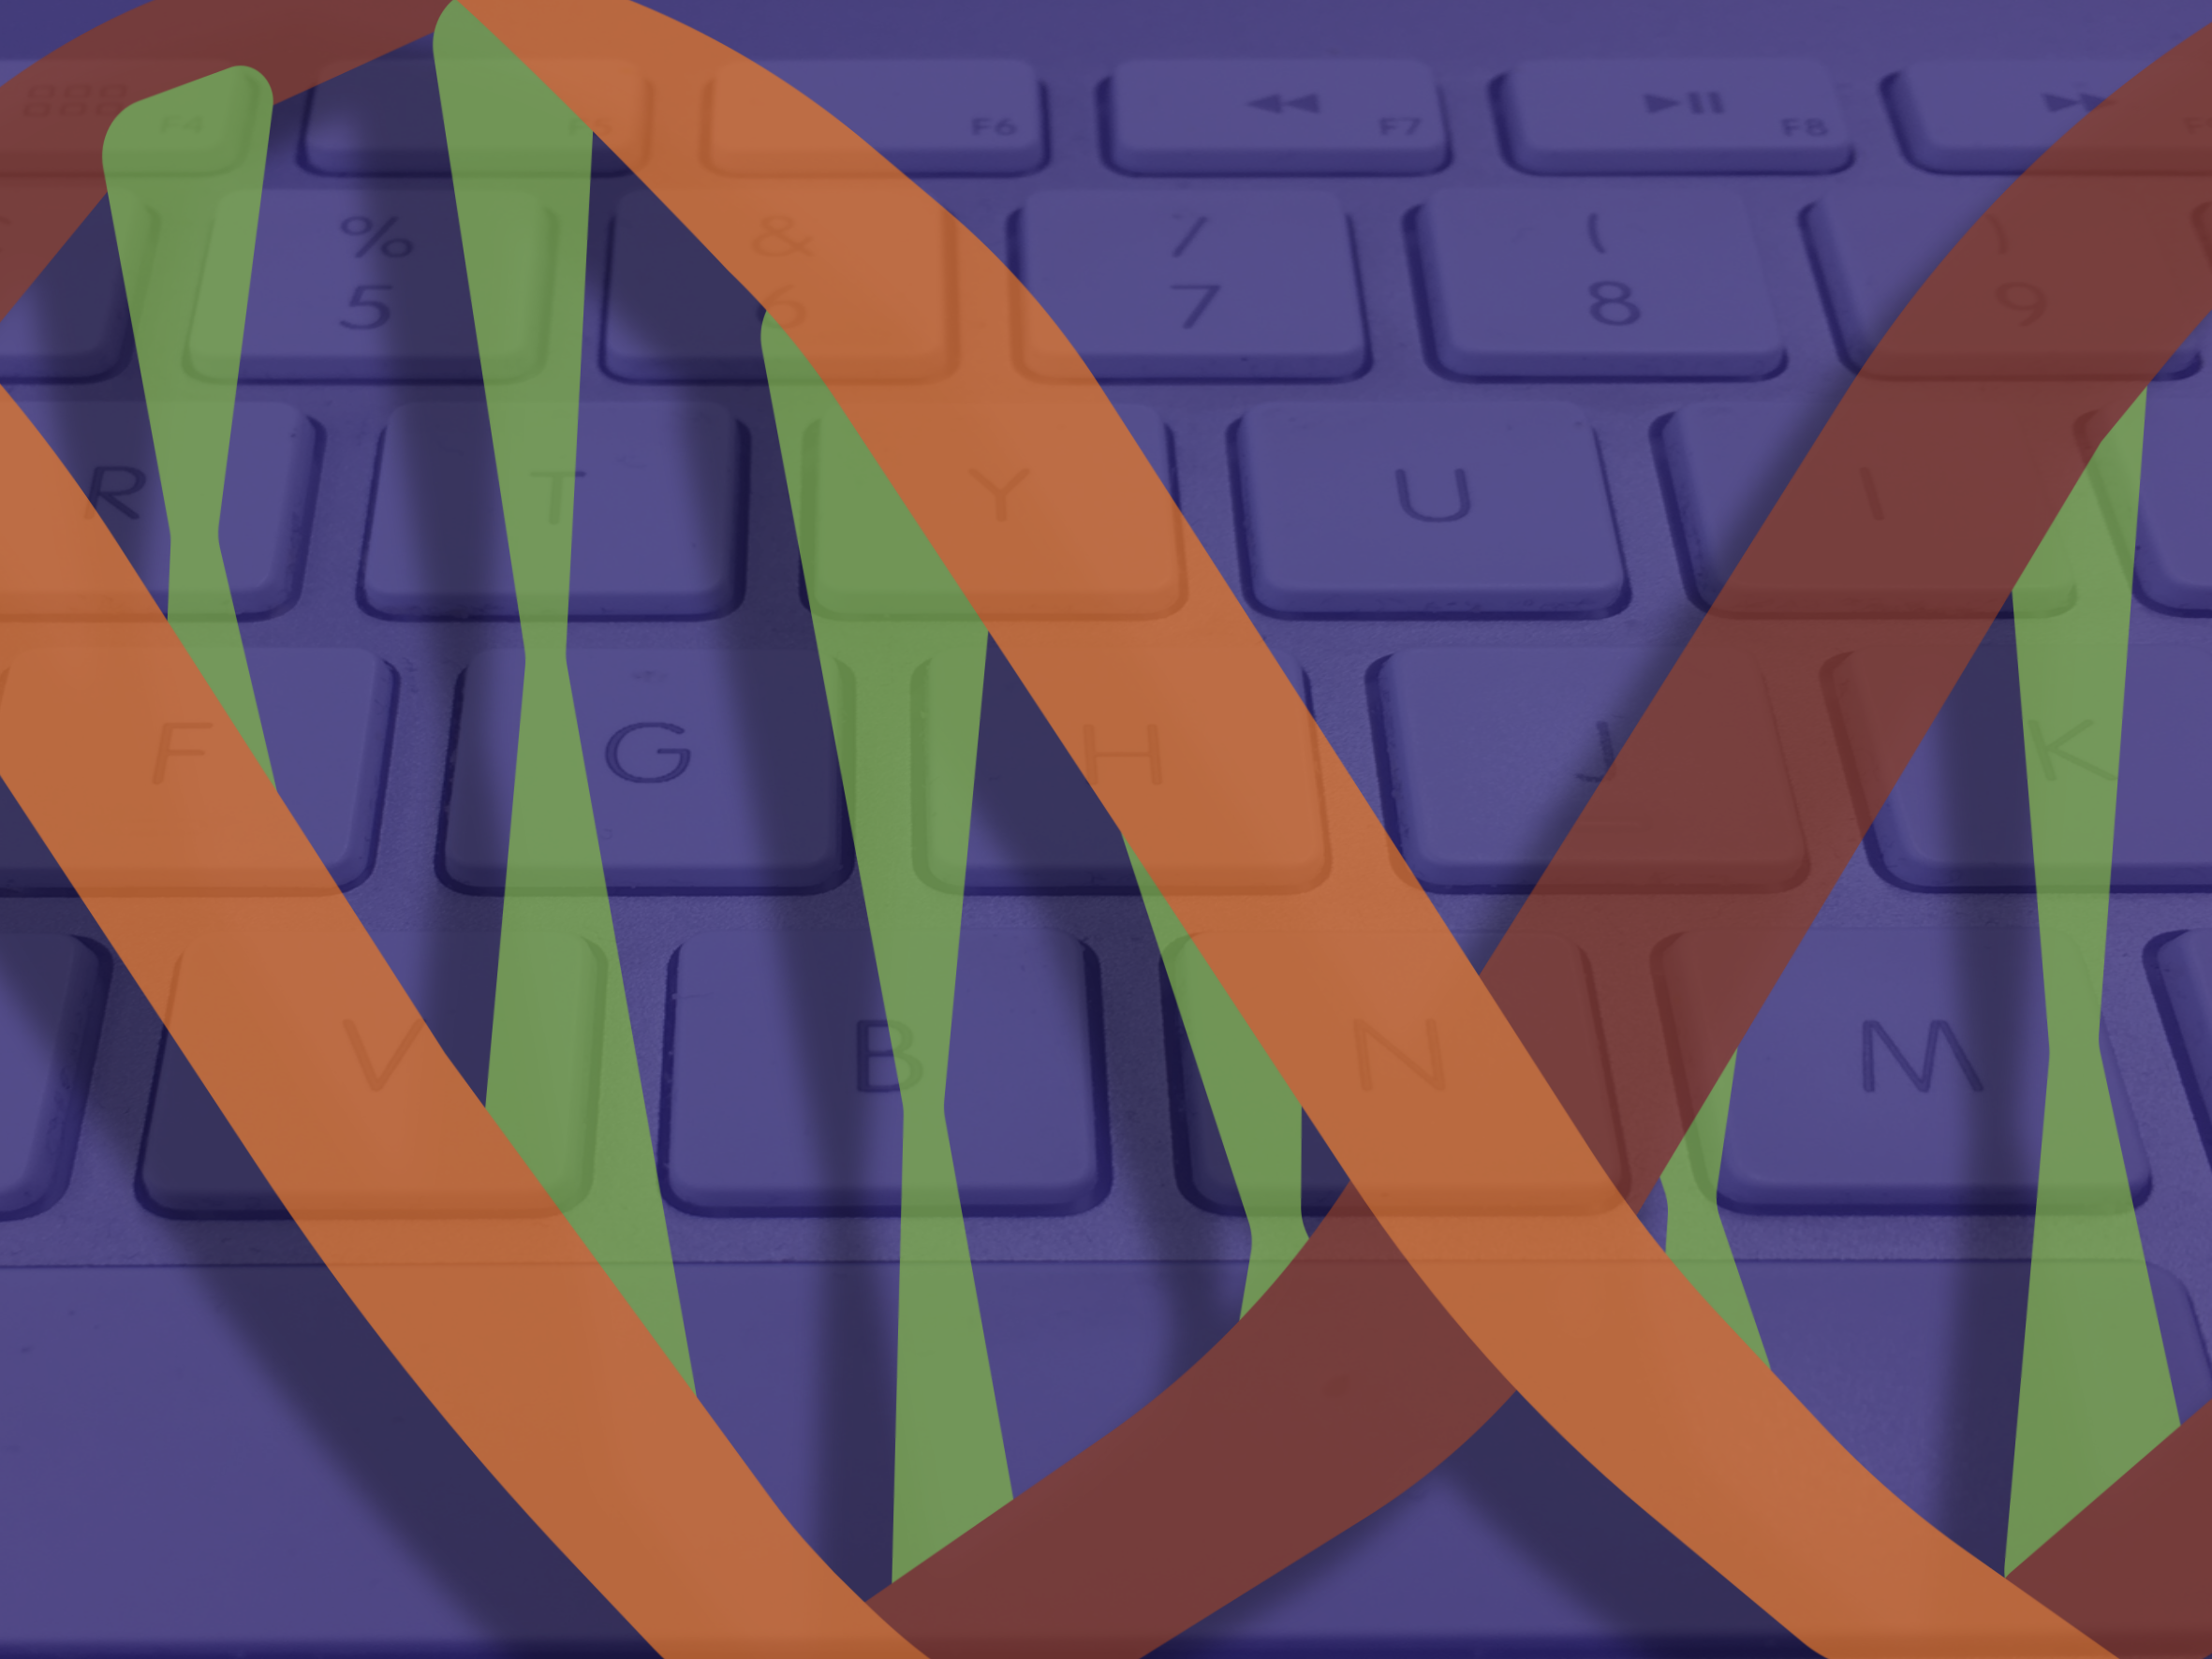
\includegraphics[width=\paperwidth,height=\paperheight]{Logos/20x15cm}} 
 
% Transcriptome: overview figure
\subsection{Overview}
\begin{frame}
\begin{center}
\begin{figure}
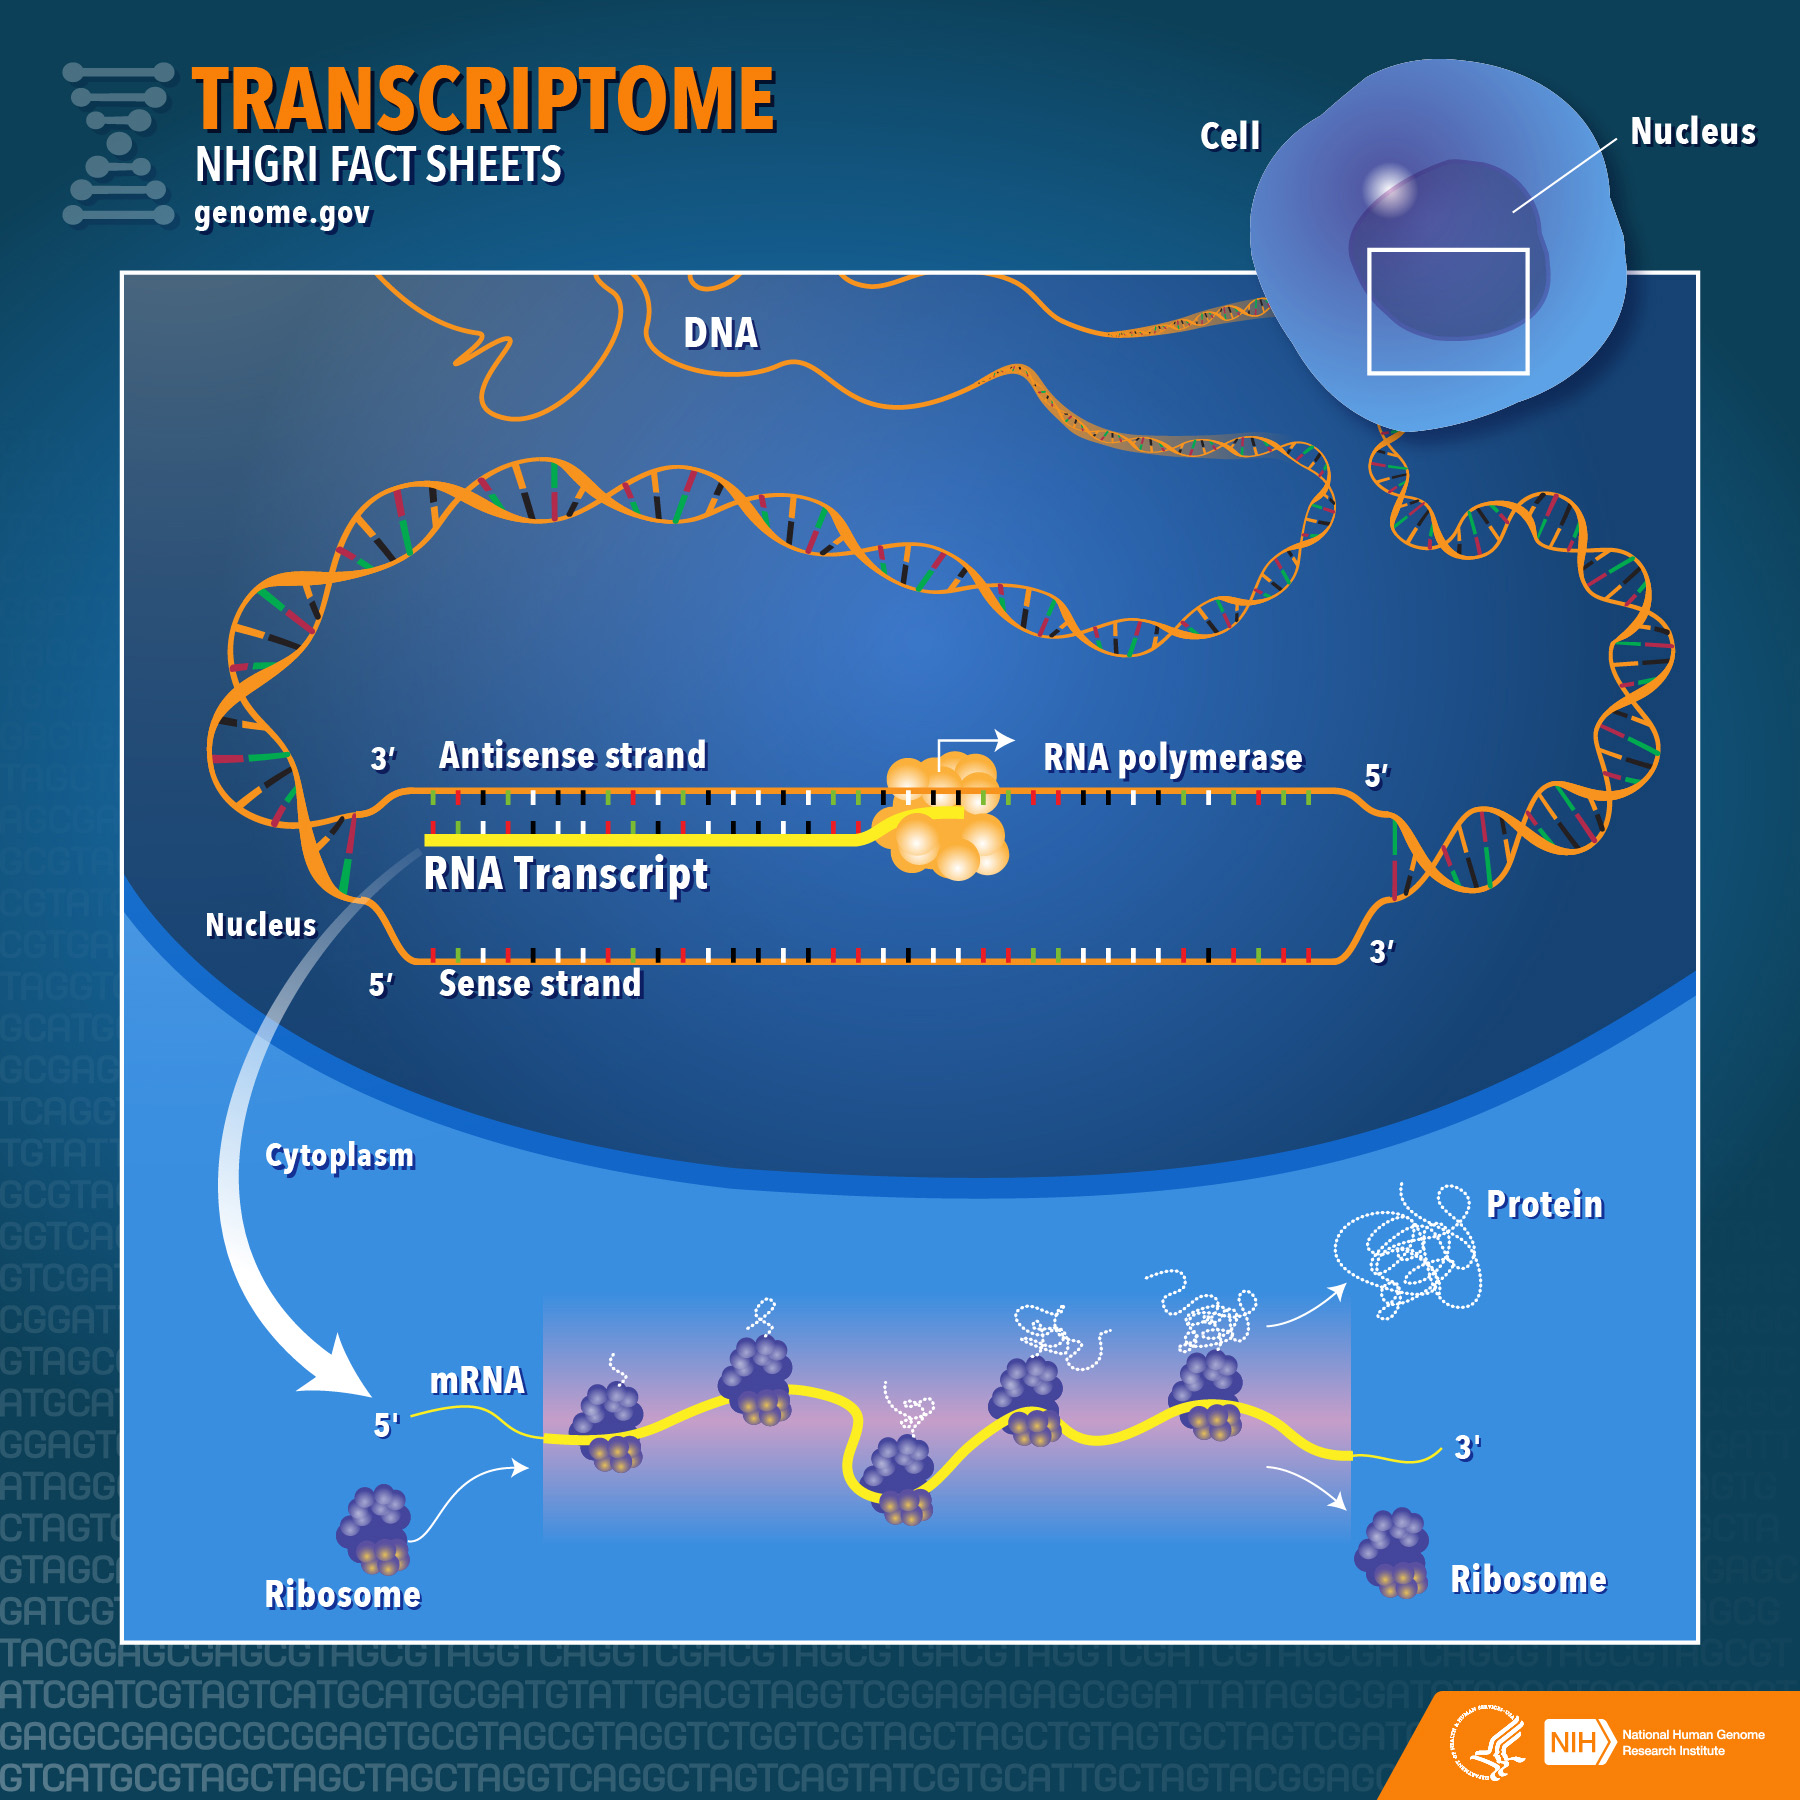
\includegraphics[height=8cm]{Images/transcriptome.jpg}
%\caption{Figure: Simplified scRNA-seq workflow [adopted from \href{http://hemberg-lab.github.io/]}{http://hemberg-lab.github.io/}}
\end{figure}
\end{center}
\end{frame}


% Why study transcriptome: quote
\begin{frame}
\begin{displayquote}
An RNA sequence mirrors the sequence of the DNA from which it was transcribed.
\end{displayquote}
\begin{displayquote}
Consequently, by analyzing transcriptome we can determine when and where each gene is turned on or off in the cells and tissues of an organism.
\end{displayquote}
\end{frame}

% Why study transcriptome: what can a transcriptome tell us about?
\begin{frame}
\begin{block}{What can a transcriptome tell us about?}
\begin{itemize}
\item gene sequences in genomes
\item gene functions
\item gene activity / gene expression
\item isoforms and allelic expression
\item fusion transcripts and novel transcripts
\item SNPs in genes
\item co-expression of genes 
\item cell-to-cell heterogeneity (scRNA-seq)
\end{itemize}
\end{block}
\end{frame}

% Why study transcriptome: what makes RNA-seq different to genome sequencing
\begin{frame}
Transcriptomes are: \newline \newline
\begin{displayquote}
dynamic, that is not the same over tissues and time points
\end{displayquote}
\begin{displayquote}
directly derived from functional genomics elements, that is mostly protein-coding genes, providing a useful functionally relevant subset of the genome, translating into smaller sequence space
\end{displayquote}
\end{frame}

% Why study transcriptome: overview
\begin{frame}
\begin{block}{Overview}
\begin{itemize}
\item \color{blue} Experimental design \color{black}(biology, medicine, statistics)
\item \color{blue} RNA extraction \color{black}(biology, biotechnology)
\item \color{blue} Library preparation (\color{black}biology, biotechnology)
\item \color{blue} High throughput sequencing \color{black}(engineering, biology, chemistry, biotechnology, bioinformatics)
\item \color{red} Data processing \color{black} (bioinformatics)
\item \color{red} Data analysis \color{black} (bioinformatics \& biostatistics)
\end{itemize}
\end{block}
\end{frame}


%% From RNA to sequence
\section{From RNA to sequence}
\subsection{Workflow}

%% From RNA to sequence: workflow v01
\begin{frame}
\begin{center}
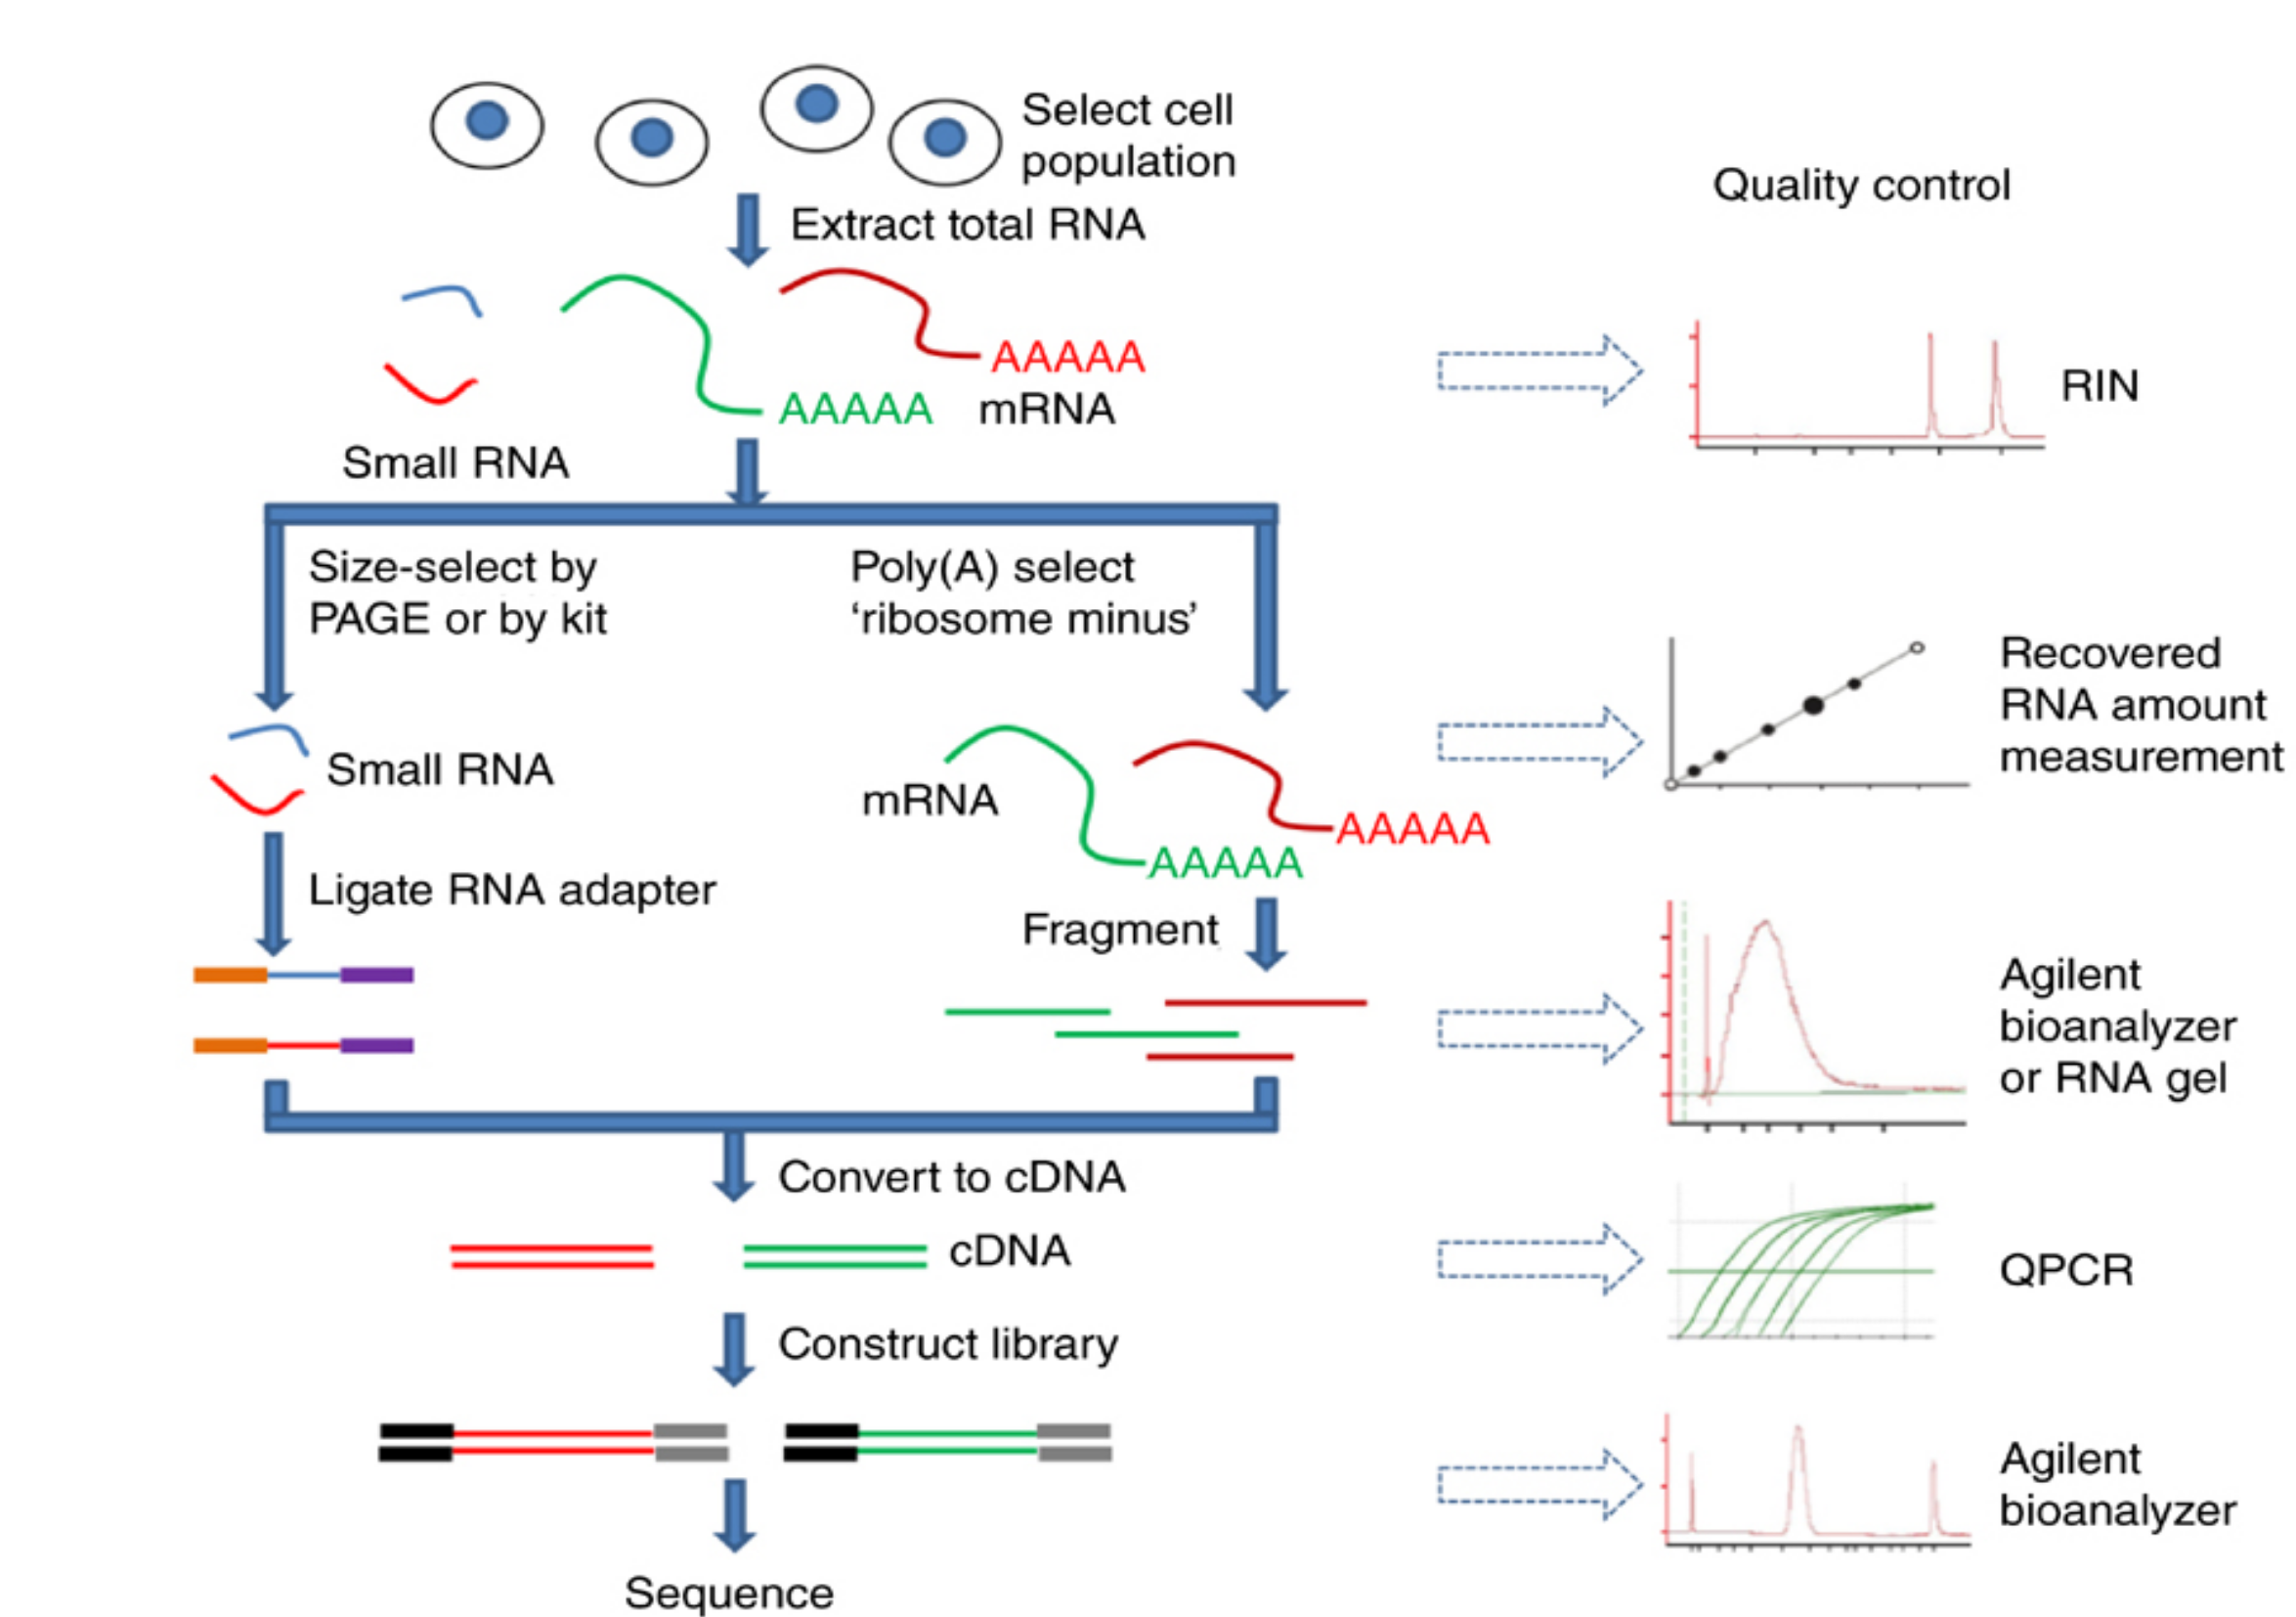
\includegraphics[height=8cm]{Images/RNA2seq.jpg}
\end{center}
\end{frame}

%% From RNA to sequence: workflow v02
\begin{frame}
\begin{center}
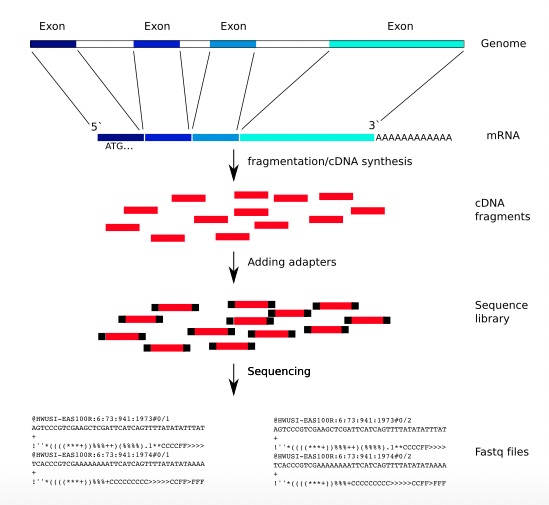
\includegraphics[height=8cm]{Images/RNA2seq2}
\end{center}
\end{frame}

\subsection{.fastq}
%% From RNA to sequence: .fastq
\begin{frame}
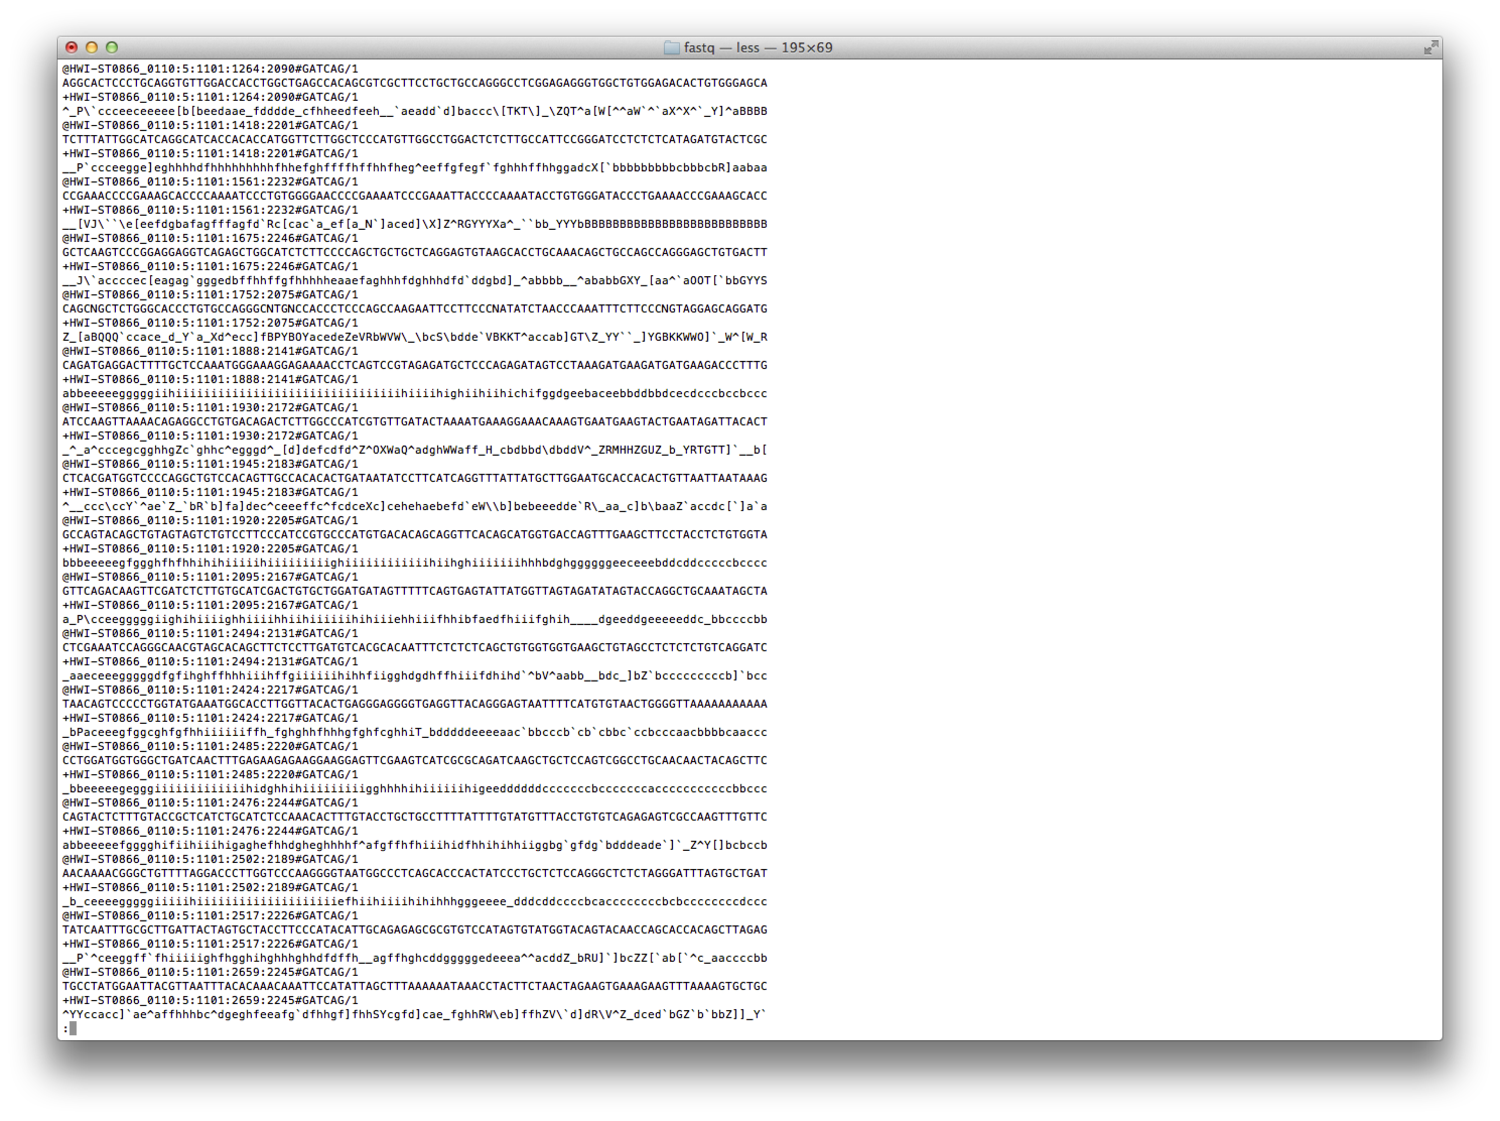
\includegraphics[width=15cm]{Images/fastqless.pdf}
\end{frame}

%% From RNA to sequence: .fastq
\begin{frame}
\begin{block}{.fastq}
@MISEQ:233:000000000-AGJP2:1:1101:15260:1358
CTGTAAATTGCCTGACTTGCTAATTGTGATTAACTTAGTTT \newline
+ \newline
BBBBBFFFFFFFGGGGGGGGGGHFFFHGHHGFFHHHHHAG
\end{block}
\begin{itemize}
\item Line1: \pause begins with a '@' character and is followed by a sequence identifier and an optional description 
\item Line2: \pause is the raw sequence letters 
\item Line3: \pause begins with a '+' character and is optionally followed by the same sequence identifier (and any description) again 
\item Line4: \pause encodes the quality values for the sequence in Line 2, and must contain the same number of symbols as letters in the sequence
\end{itemize}
\end{frame}

\subsection{Quality score}
% Understanding sequencing output (quality explanation)
\begin{frame}
\begin{columns}
\column{6cm}
\centering
\begin{block}{Phred Quality Score}
\begin{itemize}
\item Q = -10 x log P
\item where:
\begin{itemize}
\item P, probability of base calling being incorrect
\item High Q = high probability of the base being correct
\end{itemize}
\end{itemize}
\end{block}
\column{6cm}
\centering
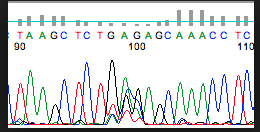
\includegraphics[width=5cm]{Images/phred.png}
\end{columns}
\begin{itemize}
\item A Phred quality score of 10 to a base means that the base is called incorrectly in 1 out of...\pause 10 times.
\item A Phred quality score of 20 to a base, means that the base is called incorrectly in 1 out of...\pause 100 times.
\item A Phred quality score of 30 to a base, means that the base is called incorrectly in 1 out of...\pause 1000 times etc...
\end{itemize}
\end{frame}


\subsection{SE/PE}
% Understanding sequencing output: SE vs PE
\begin{frame}
\begin{block}{PE, paired-end}
\begin{itemize}
\item Two .fastq files are created per sequenced library
\item The order of reads in files is identical and naming of reads is the same with the exception of the end information
\item The way of naming reads are changing over time so the read names depend on software version
\end{itemize}
\end{block}
\vspace{8mm}
\centering
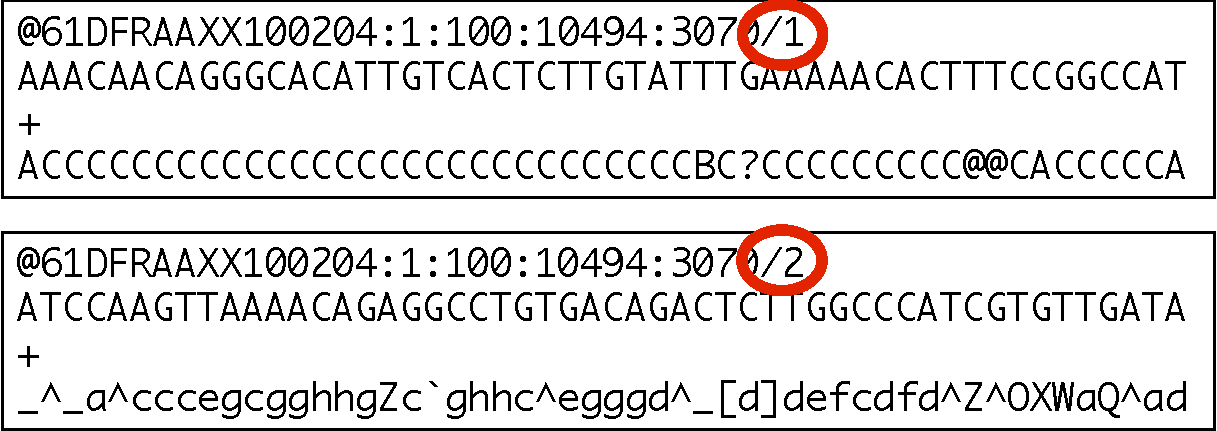
\includegraphics[width=8cm]{Images/fastqPE.pdf}
\end{frame}

\subsection{Strandness}
% Understanding sequencing output: Strandness
\begin{frame}
\footnotesize
\begin{columns}
\begin{column}{0.48\textwidth}
SE
\begin{itemize}
  \item F: the single read is in the sense (F, forward) orientation
  \item R: the single read is in the antisense (R, reverse) orientation
\end{itemize}
PE
\begin{itemize}
\item RF: first read (/1) is sequenced as anti-sense (R) \& second read (/2) is in the sense strand (F)
\item FR: first read (/1) is sequenced as sense (F) \& second read (/2) is in the antisense strand (R)
\end{itemize}
\end{column}
\begin{column}{0.48\textwidth}
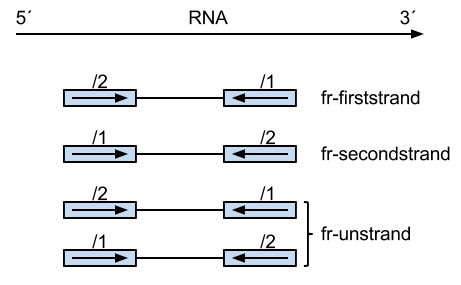
\includegraphics[width=5cm]{Images/Stranded.png}
\end{column}
\end{columns}
\end{frame}

% Reference based data analysis pipeline
\section{Reference based data analysis pipeline}
\subsection{Overview}
% Reference based data analysis pipeline: overview figure
\begin{frame}
\centering
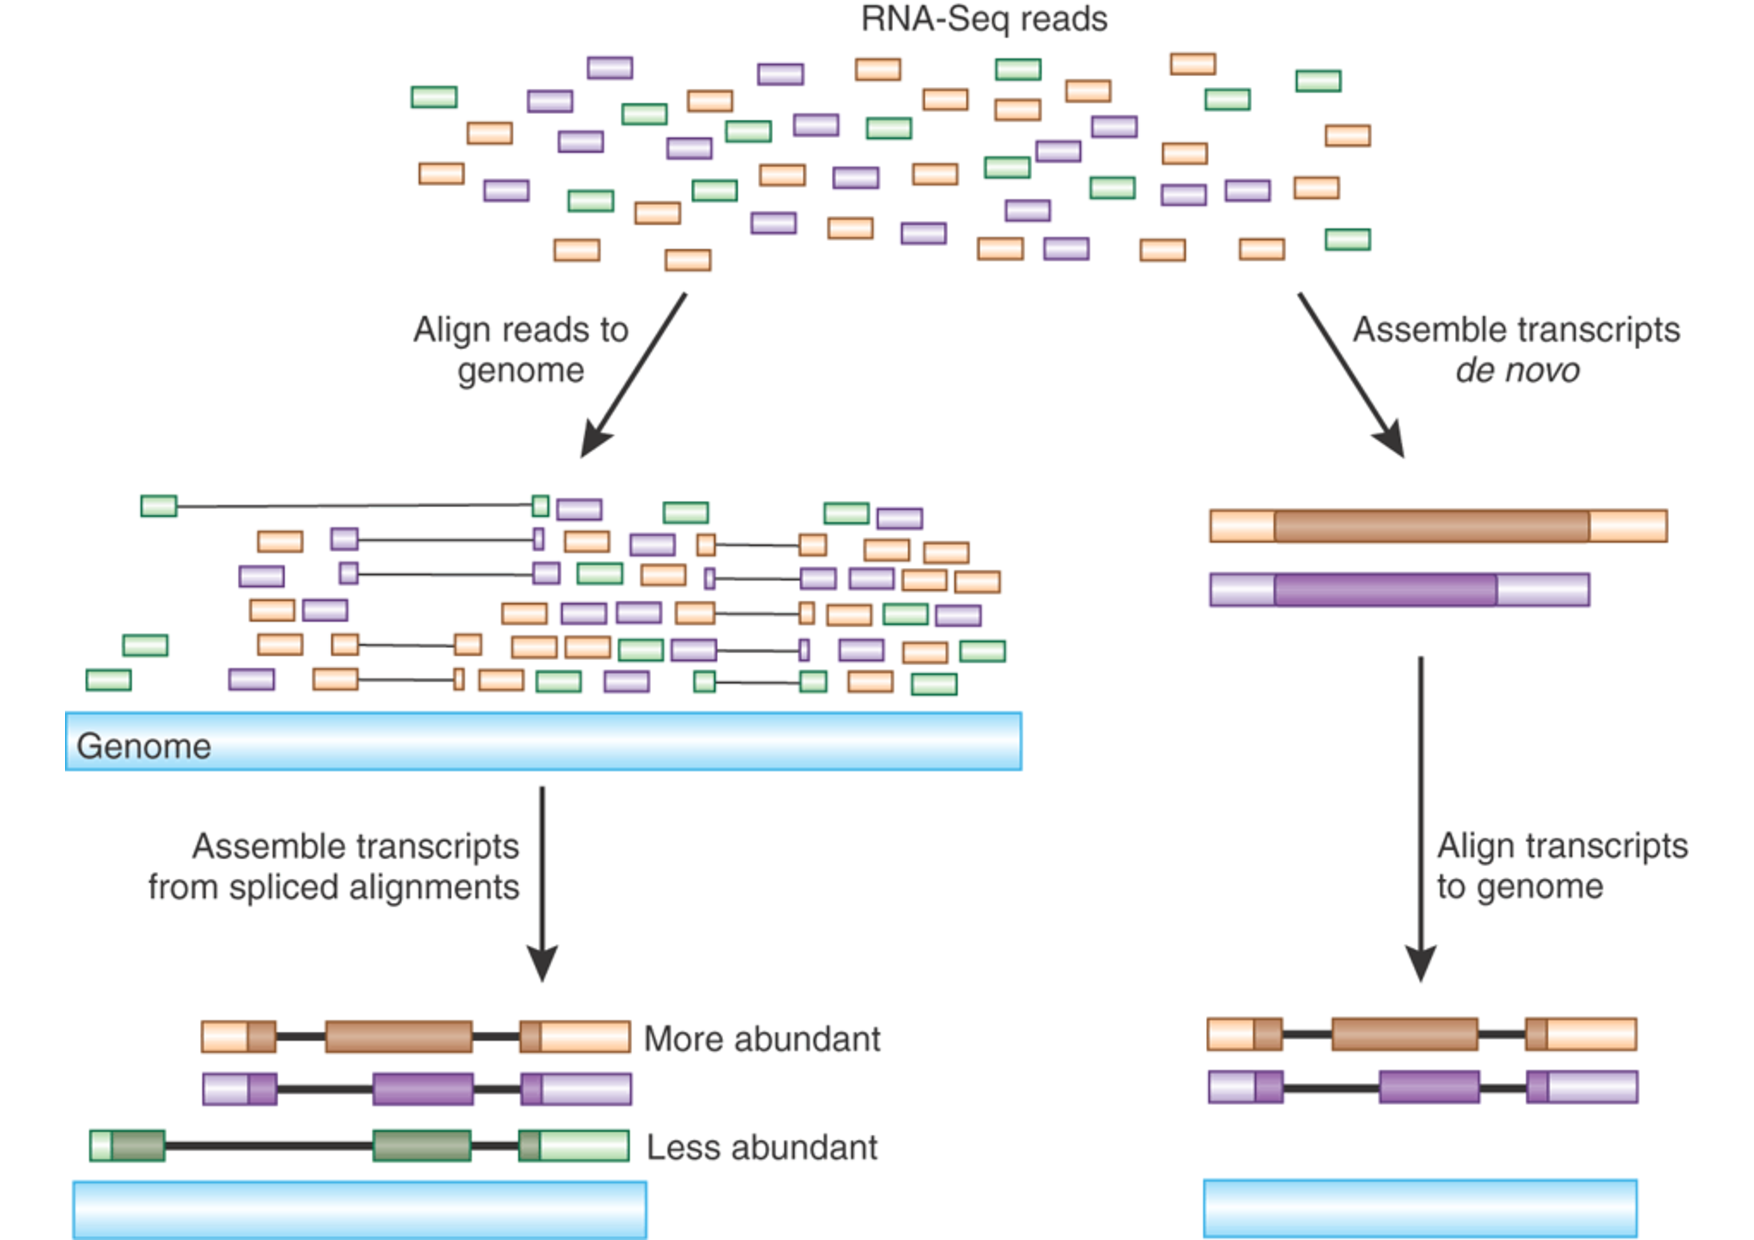
\includegraphics[width=9cm]{Images/workflows.pdf}
 % \\{\tiny{Haas \& Zody (2010), Nature Biotechnology 28, 421--423}}
\end{frame}

% Reference based data analysis pipeline: main steps
\begin{frame}
\begin{block}{Main steps}
\begin{itemize}
  \item Initial processing incl. QC
  \item Aligning reads to reference genome
  \item Counting reads
  \item Differential gene expression
  \item Further analysis
\end{itemize}
\end{block}
\end{frame}

\subsection{Initial processing}
% Reference based data analysis pipeline: filtering
\begin{frame}
\frametitle{Initial processing incl. QC}
\footnotesize
\begin{columns}
\begin{column}{0.38\textwidth}
\begin{itemize}
\item Demultiplex by index or barcode
\item Remove adapter sequences
\item Trim reads by quality
\item Discard reads by quality/ambiguity
\end{itemize}
\end{column}
\begin{column}{0.58\textwidth}
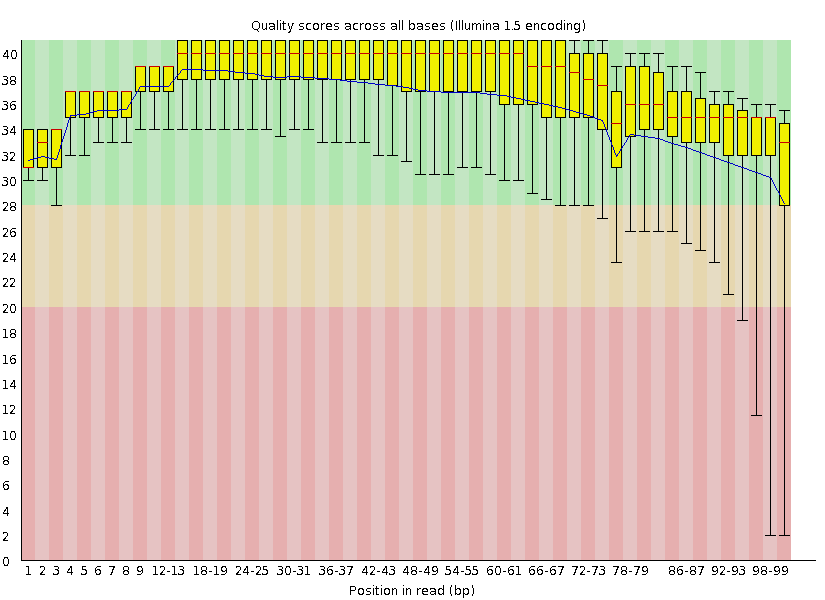
\includegraphics[width=7cm]{Images/fastq_qc_good.png}
\end{column}
\end{columns}
\vspace{5mm}
\begin{block}{Available tools}
FastQC, PRINSEQ, TRIMMOMATIC, TrimGalore, FastX, Cutadapt
\end{block}
\end{frame}

% Reference based data analysis pipeline: filtering
\begin{frame}
\frametitle{Initial processing incl. QC}
\centering
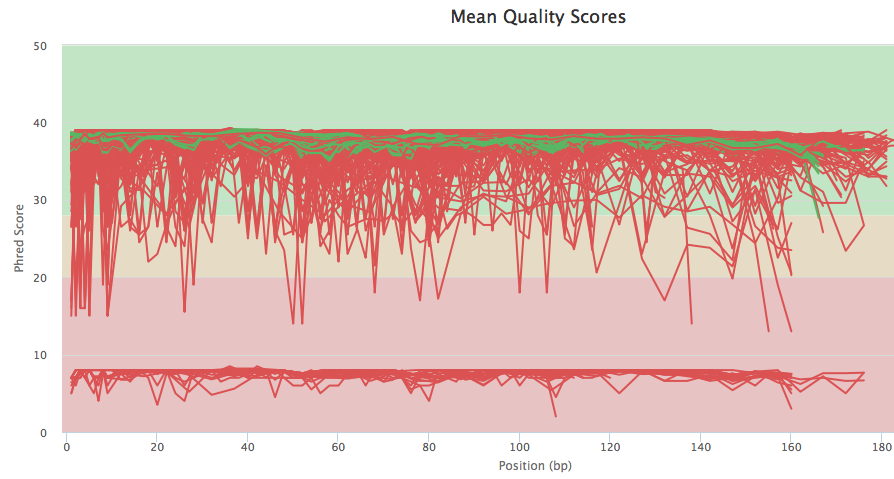
\includegraphics[width=10cm, height=4cm]{Images/fastq_qc_poor.png}
\begin{itemize}
\footnotesize
\item filtering reads for quality score, e.g. with avg. quality below 20 defined within 4-base wide sliding window
\item filtering reads for read length, e.g. reads shorter than 36 bases
\item removing artificial sequences, e.g. adapters
\end{itemize}
\end{frame}

\subsection{Aligning reads}
% Reference based data analysis pipeline: mapping
\begin{frame}
\frametitle{Aligning reads}
\centering
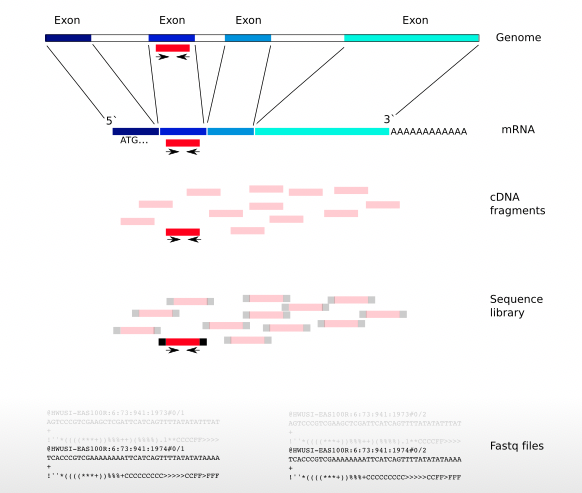
\includegraphics[height=6cm]{Images/map1.png}
\end{frame}

% Reference based data analysis pipeline: mapping
\begin{frame}
\frametitle{Aligning reads}
\centering
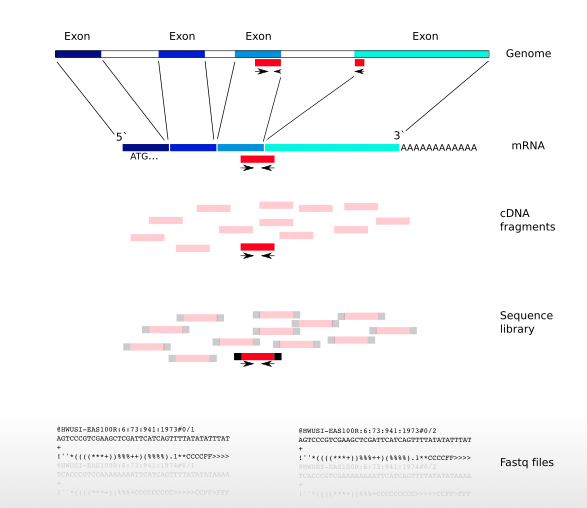
\includegraphics[height=6cm]{Images/map2.png}
\end{frame}

% Reference based data analysis pipeline: mapping aligenrs
\begin{frame}
\frametitle{Aligning reads: mappers}
\footnotesize
\begin{itemize}
  \item important to use mappers allowing for a read to be "split" between distant regions of the reference in the event that the read spans two exons
  \item lots of different aligners exists based on various algorithms e.g. brute force comparison, Burrows-Wheeler Transform, Smith-Waterman, Suffix tree
  \item usually there is a trade-off between speed versus accuracy and sensitivity
  \item usually the "biggest difference" is with default settings, most mappers will allow to optimize settings
  \item performance vary by genome complexity
\end{itemize}

\textit{A good read: Barruzo et. al. Nature Methods 14, (2017) \href{Simulation-based comprehensive bench-marking of RNA-seq aligners}{https://www.nature.com/articles/nmeth.4106}}

\vspace{5mm}
\begin{block}{Available tools}
STAR, HISAT, MapSlice2, Subread, TopHat
\end{block}
\end{frame}

% Reference based data analysis pipeline: mapping files
\begin{frame}
\frametitle{Aligning reads: reference files}
.fasta (download reference genome FASTA file)
\newline
\begin{center}
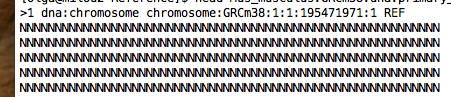
\includegraphics[width=10cm, height=1.5cm]{Images/ref.png}
\end{center}
.gtf (download the corresponding genome annotation in GTF or GFF)
\begin{center}
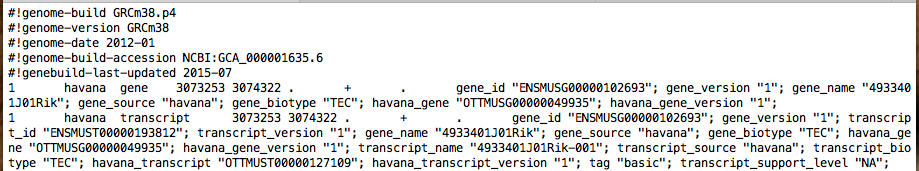
\includegraphics[width=10cm, height=2cm]{Images/ref_annotation.png}
\end{center}
\vspace{5mm}
\begin{block}{Source}
ENSEMBL, NCBI
\end{block}
\end{frame}

% % Reference based data analysis pipeline: mapping
% \begin{frame}
% \frametitle{Aligning reads}
% \centering
% 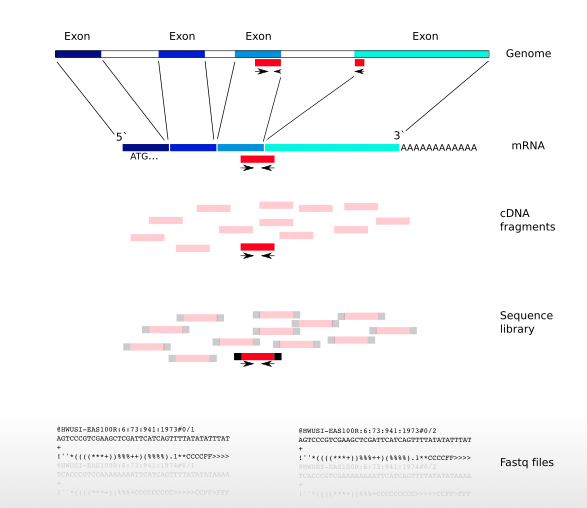
\includegraphics[height=6cm]{Images/map2.png}
% \end{frame}


% Reference based data analysis pipeline: mapping QC
\begin{frame}
\frametitle{Aligning reads: QC}
\begin{center}
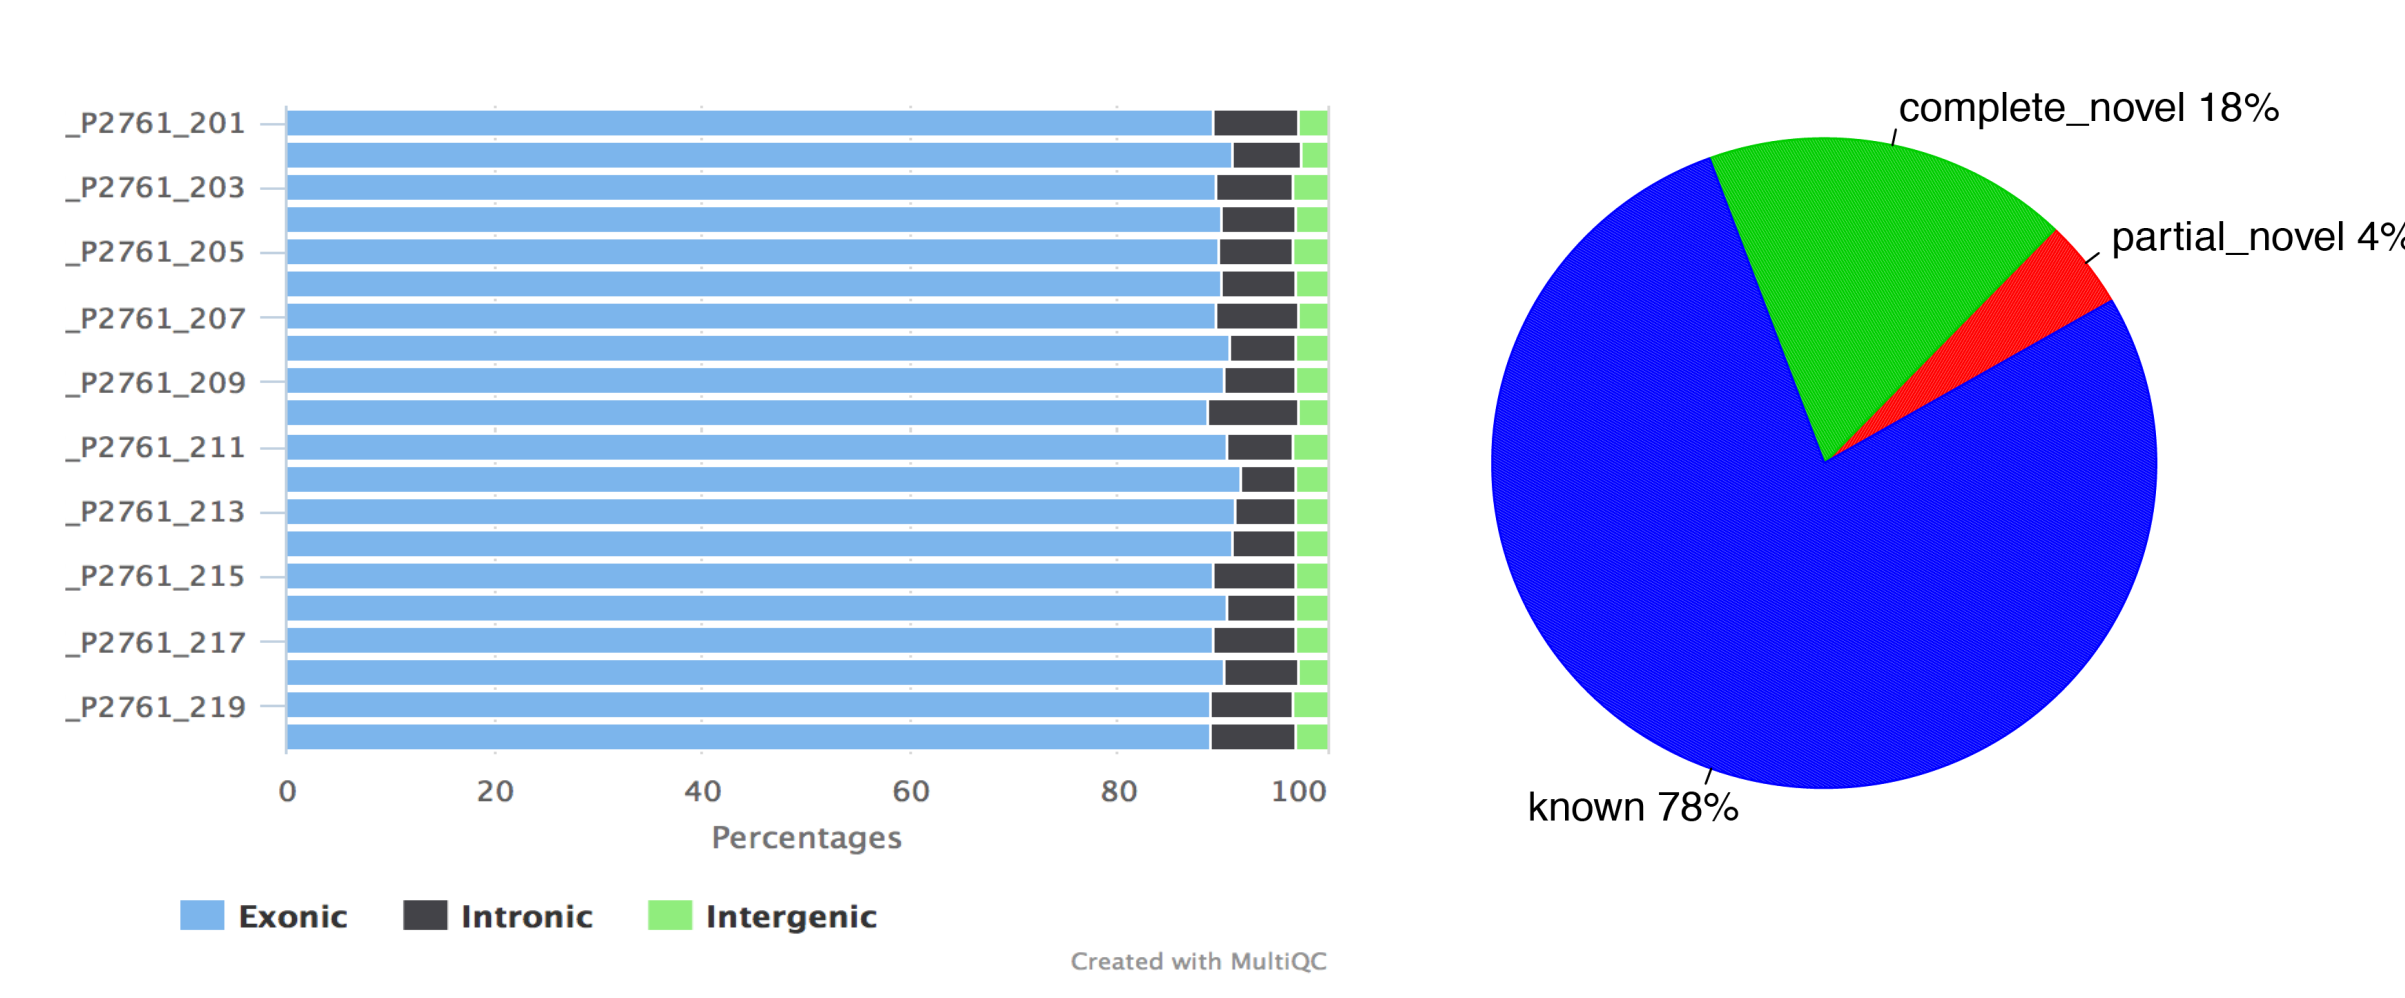
\includegraphics[width=12cm]{Images/map_qual.png}
\end{center}
Post mapping QC, e.g. reads should mostly map to known genes, most splice event should be known and canonical (GU-AG)
\end{frame}

\subsection{Counting}
% Reference based data analysis pipeline: counting
\begin{frame}
\frametitle{Counting reads}
\begin{center}
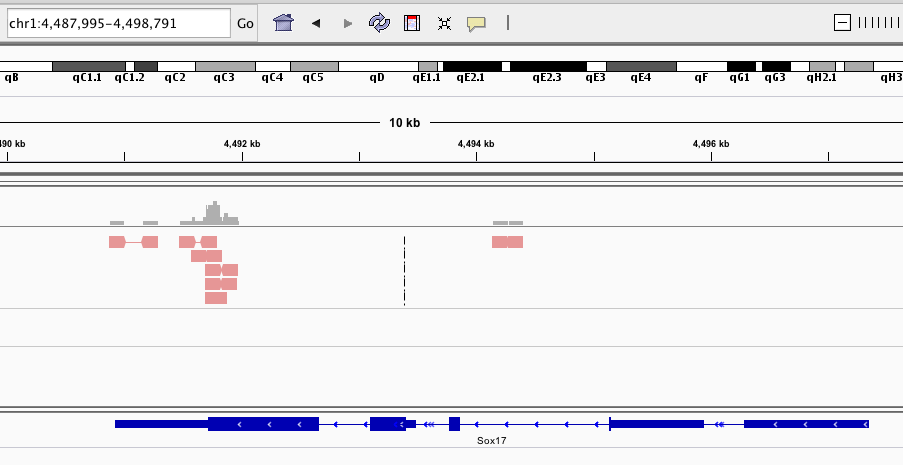
\includegraphics[width=10cm, height=5cm]{Images/counts_IGV.png}
\end{center}
\begin{block}{Available tools}
HTSeq, featureCounts, R
\end{block}
\end{frame}

% Reference based data analysis pipeline: counting
\begin{frame}
\frametitle{Counting reads}
\centering
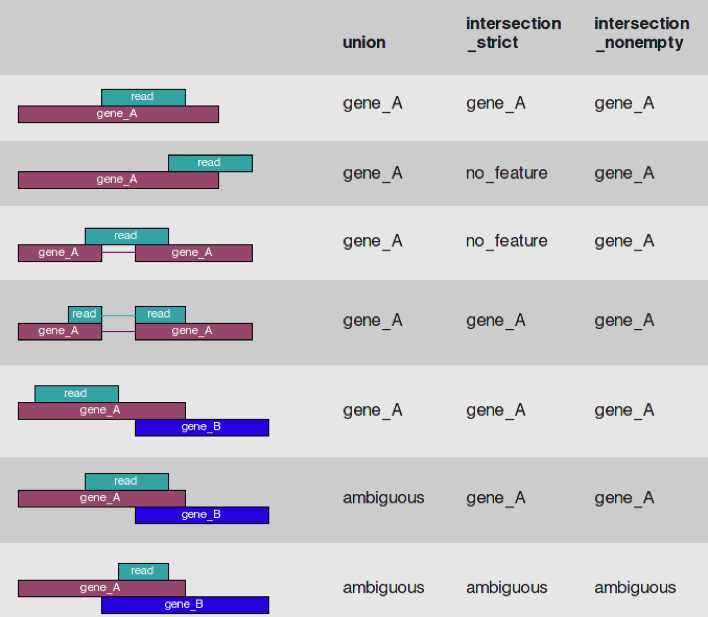
\includegraphics[width=7cm]{Images/counts_HTseq.png}
  \\{\tiny{from: http://www-huber.embl.de/users/anders/HTSeq/doc/count.html}}
\end{frame}

% Reference based data analysis pipeline: counting
\begin{frame}
\frametitle{Counting reads}
\begin{center}
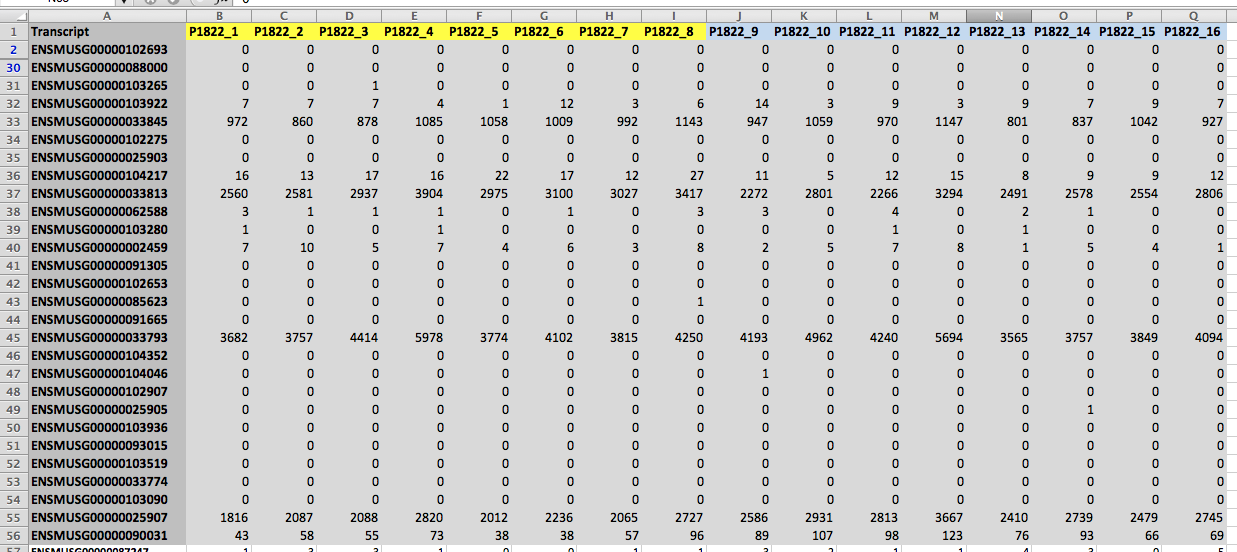
\includegraphics[width=12cm, height=7cm]{Images/counts_table.png}
\end{center}
\end{frame}

% Reference based data analysis pipeline: normalizing counting
\begin{frame}
\frametitle{Normalizing counts}
\begin{displayquote}
Gene counts depend e.g. on sequencing depth a sample and on the sequence lighten of the gene/transcript. Raw read counts cannot be used to compare gene expression across libraries. 
\end{displayquote}
\begin{block}{Normalization methods}
\begin{itemize}
\item CPM, counts per million, accounts for sequencing depth
\item RPKM/FPKM, Reads/Fragments Per Kilobase Per Milion accounts for sequencing depth and transcript length
\item TMM, Trimmed Mean of M-values, accounts for sequencing depth and transcript length and composition of the RNA population
\item any few other using scaling factors
\end{itemize}
\end{block}
\end{frame}

\subsection{Differential expression}
% Reference based data analysis pipeline: differential expression model
\begin{frame}
\frametitle{Differential gene expression}
\begin{center}
\begin{figure}
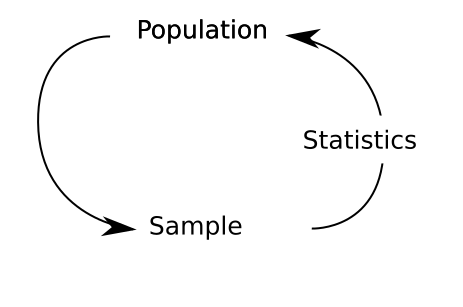
\includegraphics[width=5cm]{Images/stats.png}
\end{figure}
$Outcome_i=(Model_i)+error_i$
\end{center}
\begin{itemize}
\footnotesize
\item we collect data on a \underline{\textit{sample}} from a much larger \underline{\textit{population}}. \underline{\textit{Statistics}} lets us to make inferences about the population from which it was derived
\item we try to predict the outcome given a model fitted to the data
\end{itemize}
\end{frame}

\begin{frame}
\frametitle{Differential gene expression}
\begin{columns}
\begin{column}{0.48\textwidth}
\begin{flushright}
\footnotesize
$t=\frac{x_1-x_2}{s_p\sqrt{\frac{1}{n_1}+\frac{1}{n_2}}}$
\end{flushright}
\begin{knitrout}
\definecolor{shadecolor}{rgb}{0.969, 0.969, 0.969}\color{fgcolor}
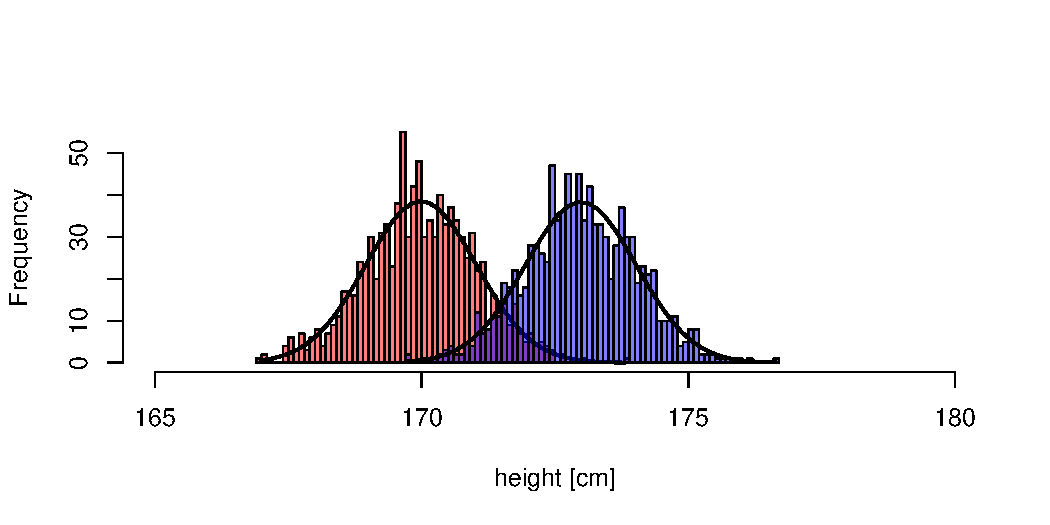
\includegraphics[width=\maxwidth]{figure/ttest-1} 

\end{knitrout}
\end{column}
\begin{column}{0.48\textwidth}
\footnotesize
in RNA-seq case:
\begin{itemize}
\item we take the normalized read counts 
\item and we perform statistical analysis to discover quantitative changes in expression levels between experimental groups
\item e.g. to decide whether, for a given gene, an observed difference in read counts is significant, that is, whether it is greater than what would be expected just due to natural random variation.
\end{itemize}
\end{column}
\end{columns}
\end{frame}

% RNA-seq mapping based approach: differential expression
\begin{frame}
\frametitle{Differential expression}
\begin{displayquote}
Usually, reads counts do not usually follow normal distribution \& we work with low number of replicates or samples per group
\end{displayquote}
\begin{block}{DE methods}
\begin{itemize}
\item Discrete distribution models, e.g. edgeR, DESeq2
\item Continuous discrete models, e.g. t-test
\item Non-parametric model, e.g. SAMseq 
\end{itemize}
\end{block}
\begin{center}
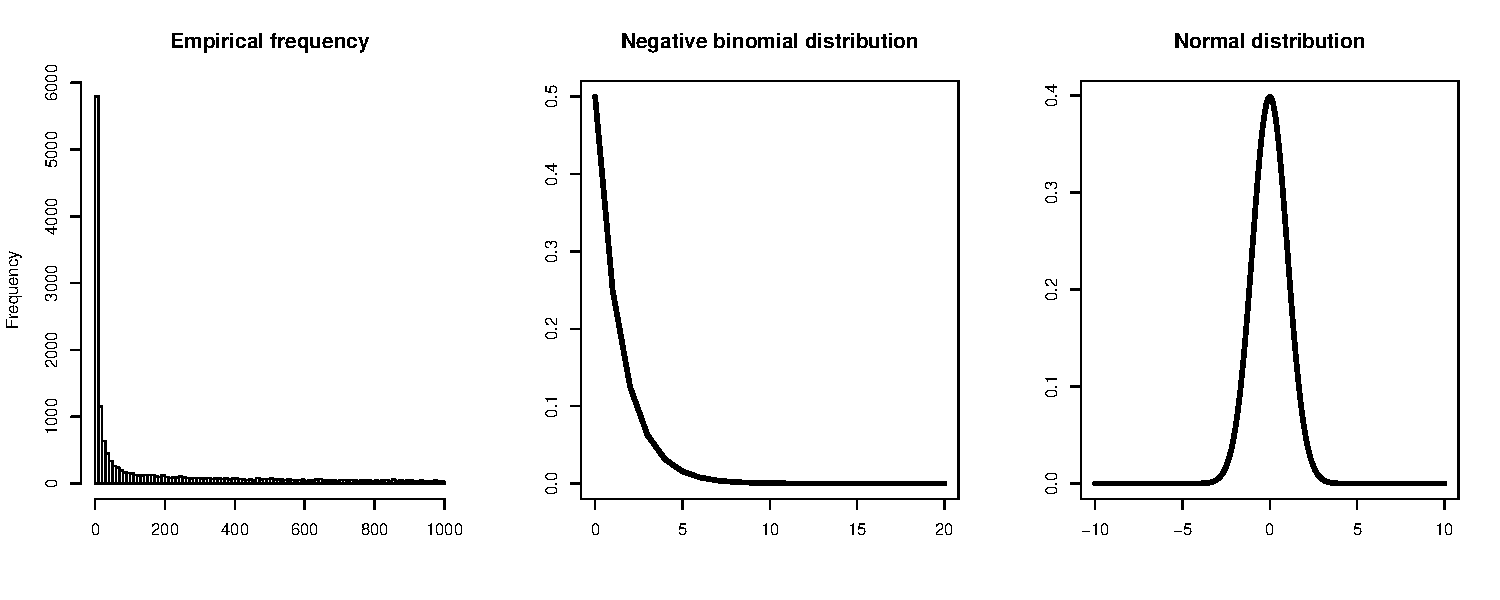
\includegraphics[width=10cm, height=3cm]{Images/DE_distribution.pdf}
\end{center}
\end{frame}


% RNA-seq mapping based approach: differential expression
\begin{frame}
\frametitle{Differential expression}
\vspace{1cm}
\begin{center}
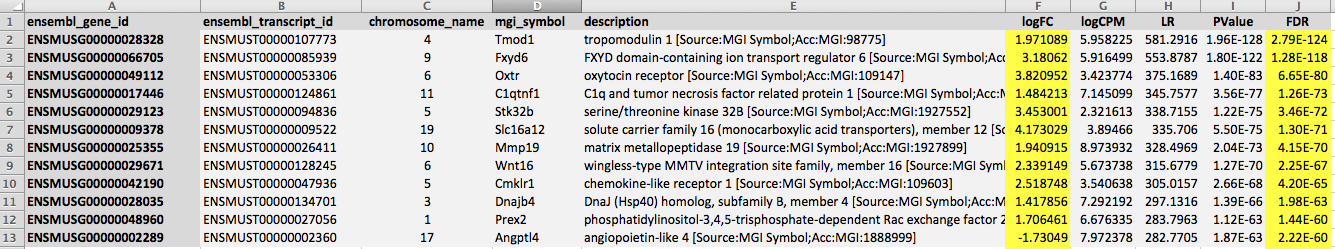
\includegraphics[width=12cm, height=3cm]{Images/DE_table.png}
\end{center}
\begin{displayquote}
\footnotesize
The likelihood of observing a significant p-value increases as we do more tests, i.e. testing more than one gene. Modern FDR adjustment techniques take into account of background expectation of a uniformly distributed p-values and adjust their values accordingly to how significantly different things are, so the p-values from multiple testing can be interpreted more accurately. 
\end{displayquote}
\end{frame}

% RNA-seq mapping based approach: differential expression exons
\begin{frame}
\frametitle{Differential expression}
\begin{center}
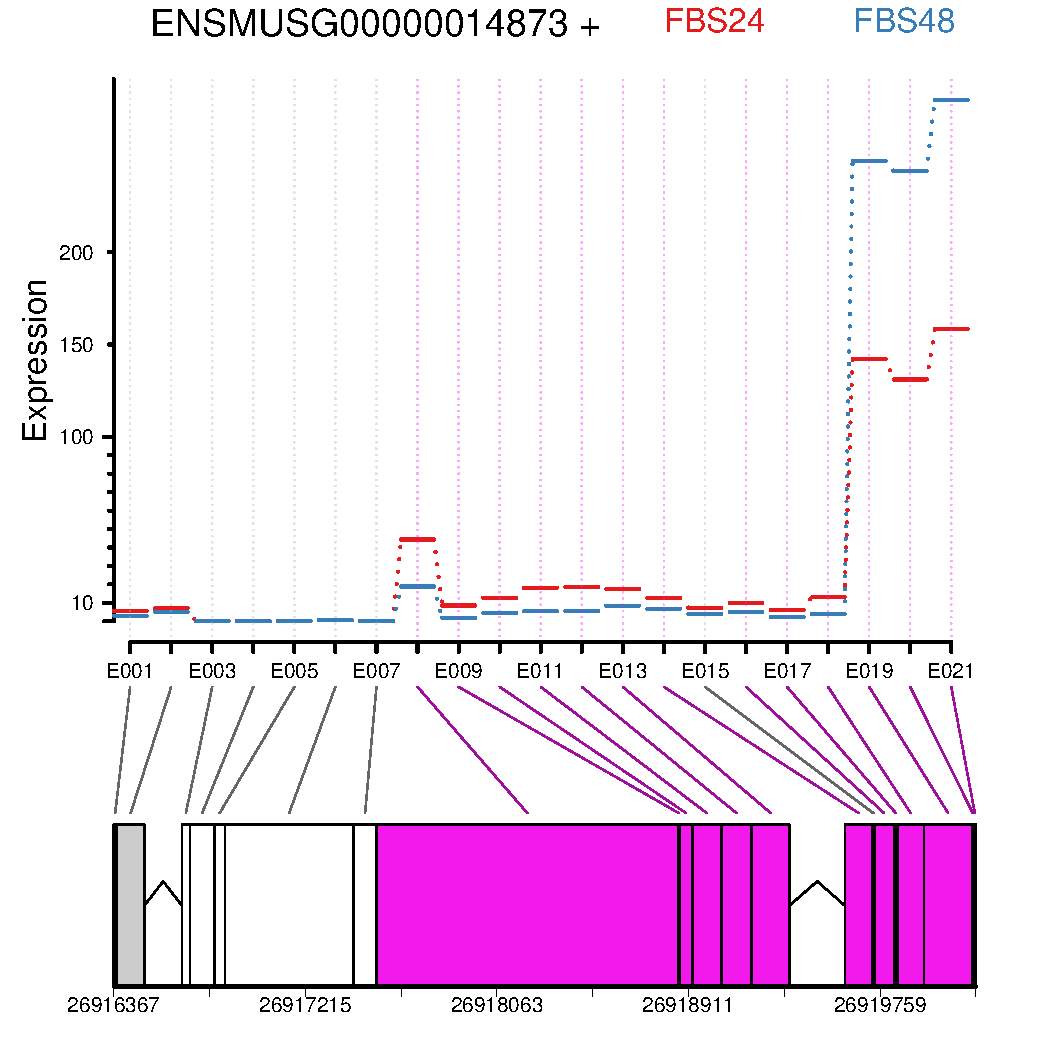
\includegraphics[width=12cm, height=6cm]{Images/DE_exon.pdf}
\end{center}
\begin{block}{Available tools}
edgeR, DEXSeq
\end{block}
\end{frame}

\subsection{Further analysis}
% RNA-seq mapping based approach: further analysis
\begin{frame}
\frametitle{Further analysis}
\begin{center}
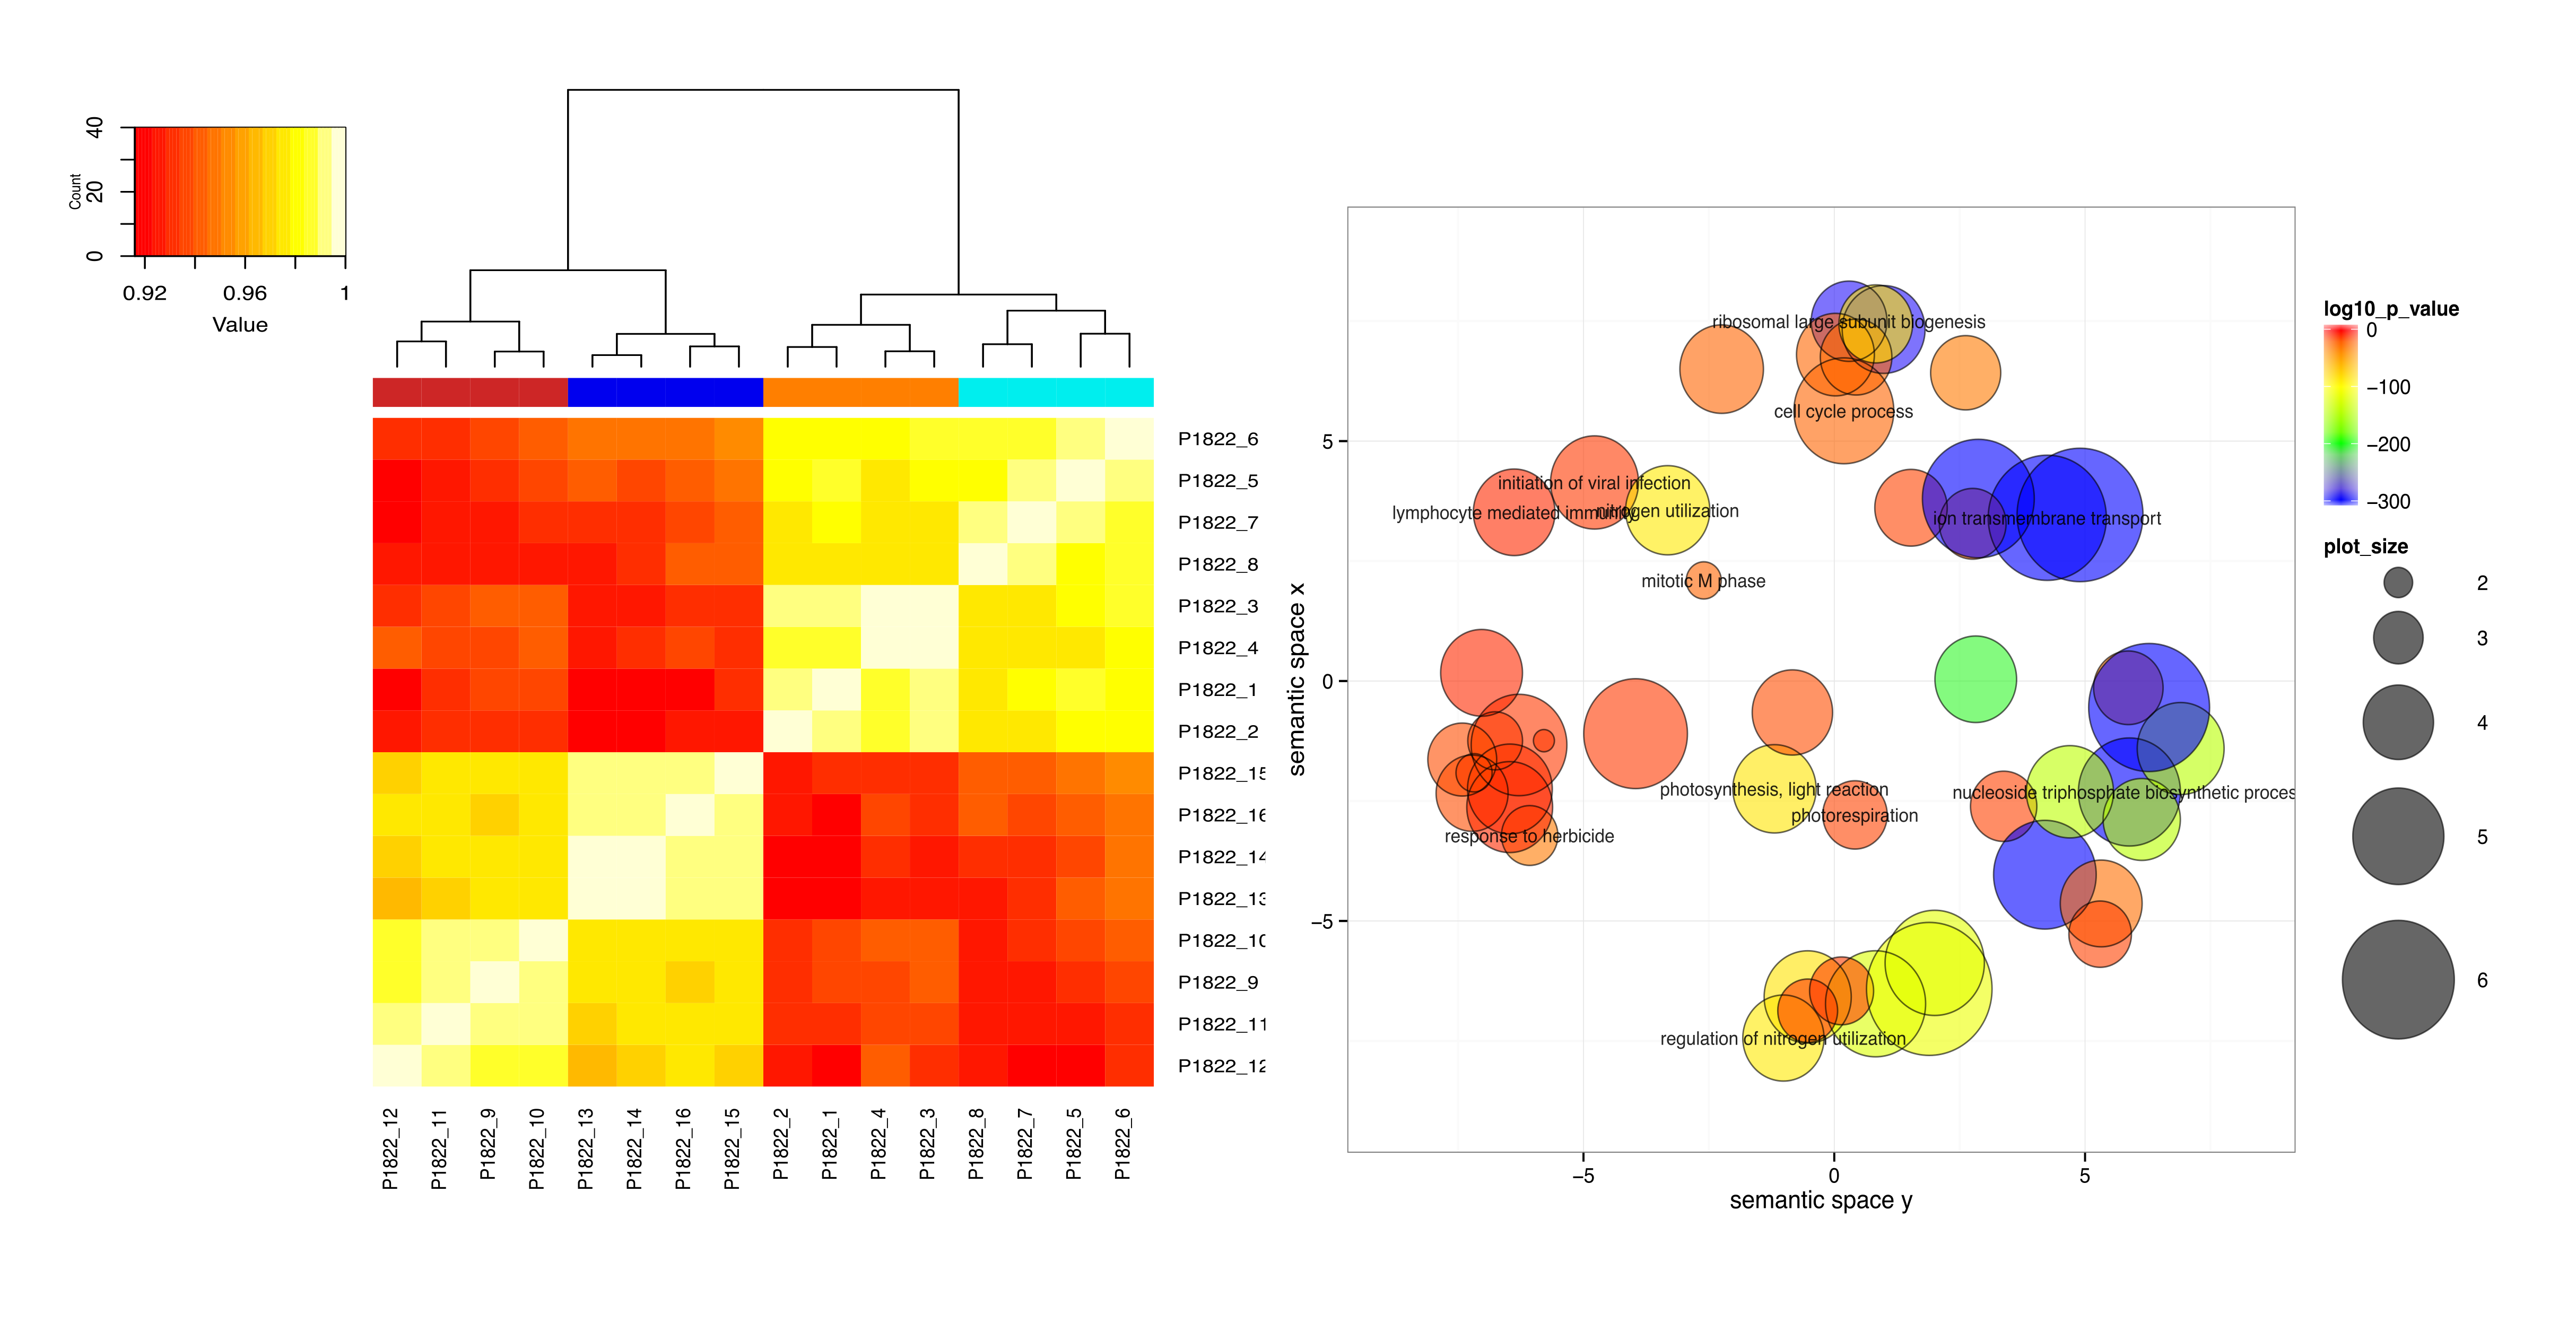
\includegraphics[width=8cm]{Images/DE_beyond.png}
\end{center}
\begin{itemize}
\item Annotating the results e.g. with gene symbols, GO terms
\item Visualizing the results, e.g. Volcano plots
\item Gene set analysis etc...
\end{itemize}
\begin{block}{Available tools}
bioMart (R), DAVID, GOrilla, REVIGO, ClustVis...
\end{block}
\end{frame}

\section{What about de-novo assembly of transcriptomes?}
\subsection{Overview}
% de-novo: overview
\begin{frame}
\centering
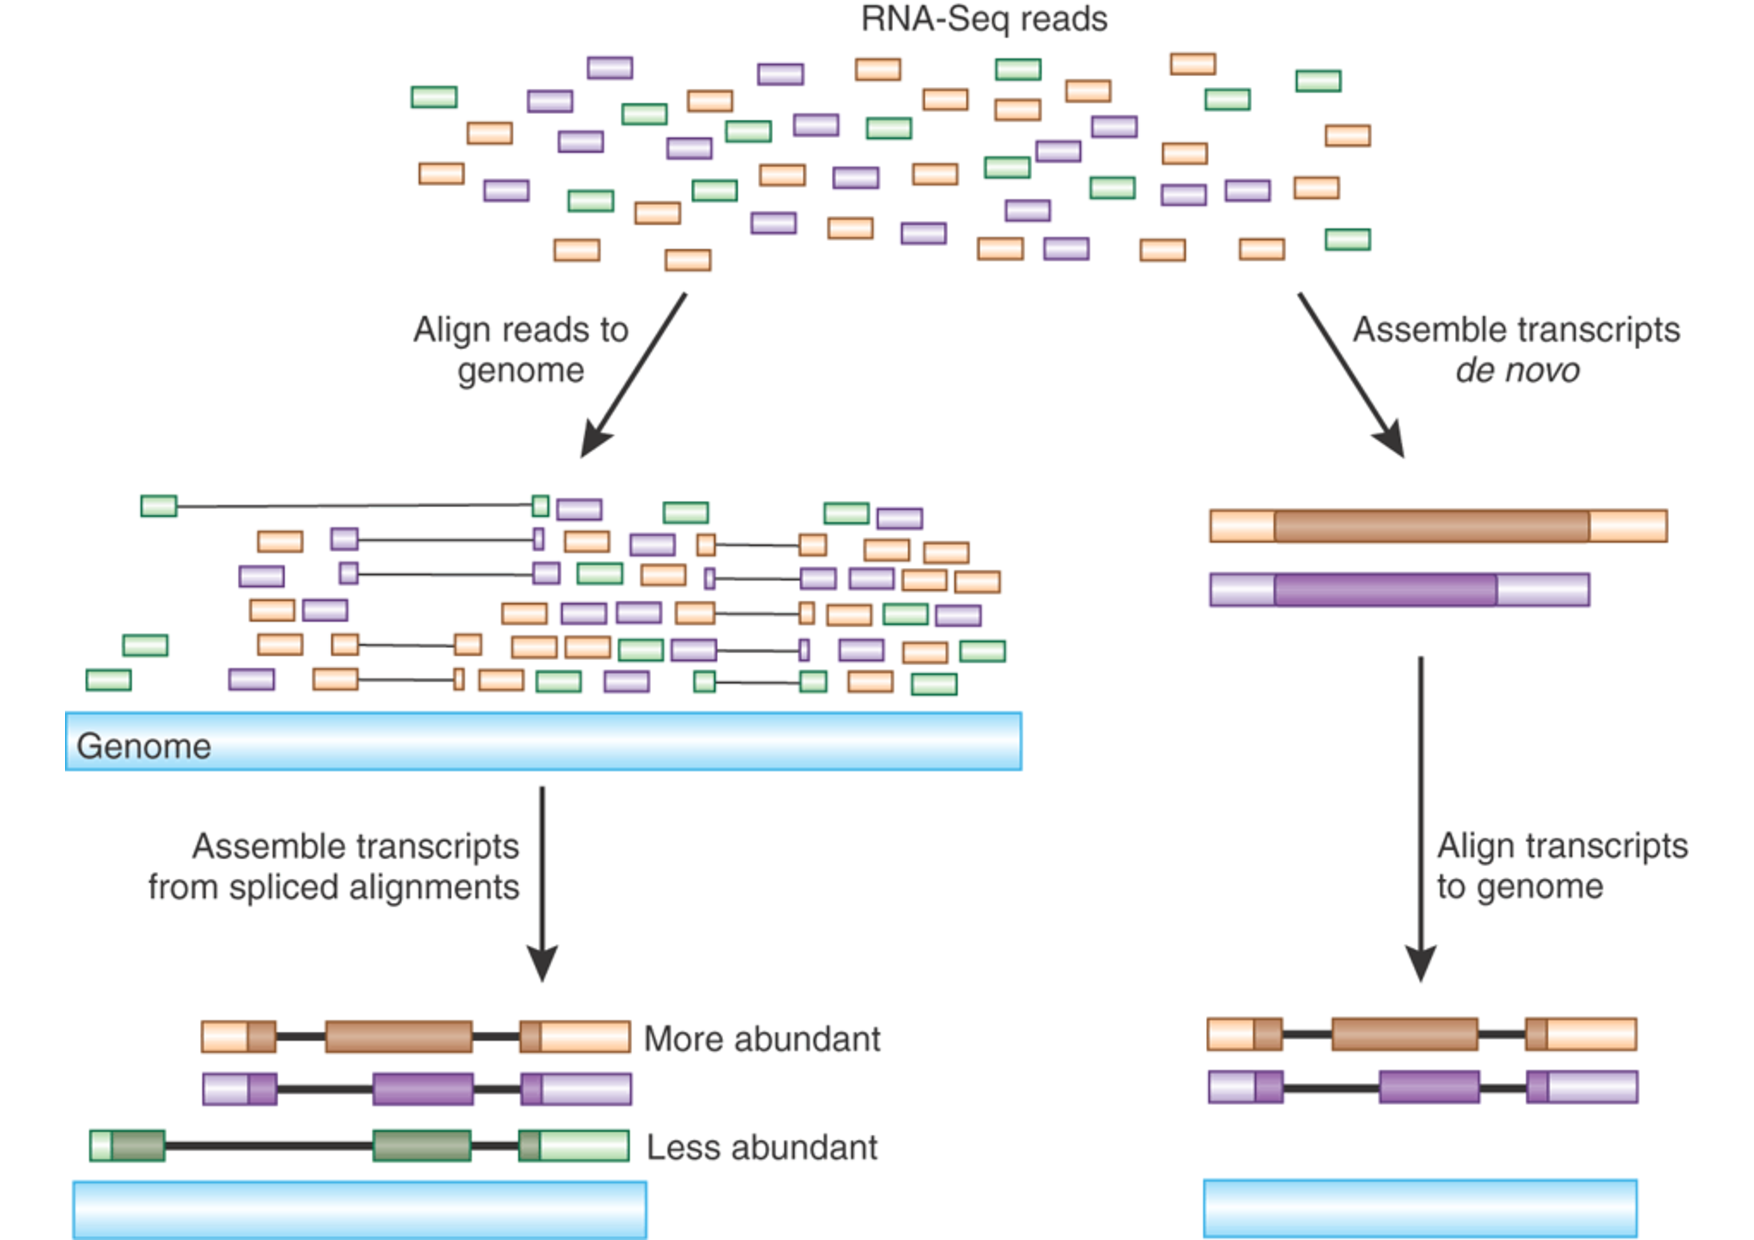
\includegraphics[width=9cm]{Images/workflows.pdf}
\end{frame}

% de-novo: overview
\subsection{Building a reference transcriptome}
\begin{frame}
Building a reference transcriptome
\footnotesize
\begin{itemize}
 \item alternative strategy when well-assembled reference genome from a relatively recently diverged organism is not available
 \item primary goal: assembling a transcriptome \textit{de novo} to reconstruct a set of contigous sequences (contigs) presumed to reflect accurately a large portion of the RNAs actually transcribed in the cells
\end{itemize}
\vspace{5mm}
not a trivial task, because 
\begin{itemize}
\scriptsize
 \item a limited amount of information about the original gene transcripts is retained in the short reads produced by a sequencer
 \item genes show different levels of gene expression (uneven coverage)
 \item more sequencing depth is needed to represent less abundant genes and rare events
 \item reads from the same transcript must be placed together in the face of variants introduced by polymorphism and sequencing errors
 \item and the process must assemble reads from different but often similar, paralogous transcripts as separate contigs
\end{itemize}
\end{frame}

% de-novo: overview
\begin{frame}
\begin{displayquote}
\footnotesize
Solutions to sequence assembly arose from the field of mathematics known as graph theory. These approaches were designed with genome assembly in mind but have been adapted for transcriptome assembly as necessary. Most of them are based on de Brujin graphs. 
\end{displayquote}
\begin{block}{Available tools}
\begin{itemize}
\footnotesize
\item Velvet/Oases: Velvet constructs de Bruijn graphs, simplifies the graphs, and corrects the graphs for errors and repeats. Oases post-processes Velvet assemblies with different k-mer sizes
\item Trans-ABySS: much like the Velvet/Oases model, Trans-ABySS (Robertson et al. 2010) takes multiple ABySS assemblies (Simpson et al. 2009) produced from a range of k-mer sizes to optimize transcriptome assemblies in the face of varying coverage across transcripts
\item Trinity: "Inchworm" builds initial contigs by finding paths through k-mer graphs. "Chrysalis" groups these contigs together and builds de Bruijn graphs for these groups, in which the overlaps are nodes and the k-mers connecting edges. "Butterfly" simplifies the graphs when possible, then reconciles the graphs with original reads to output individual contigs representative of unique splice variants and paralogous transcripts
\end{itemize}
\end{block}
\vspace{5mm}
\end{frame}

\begin{frame}
\begin{center}
\begin{columns}
\begin{column}{0.48\textwidth}
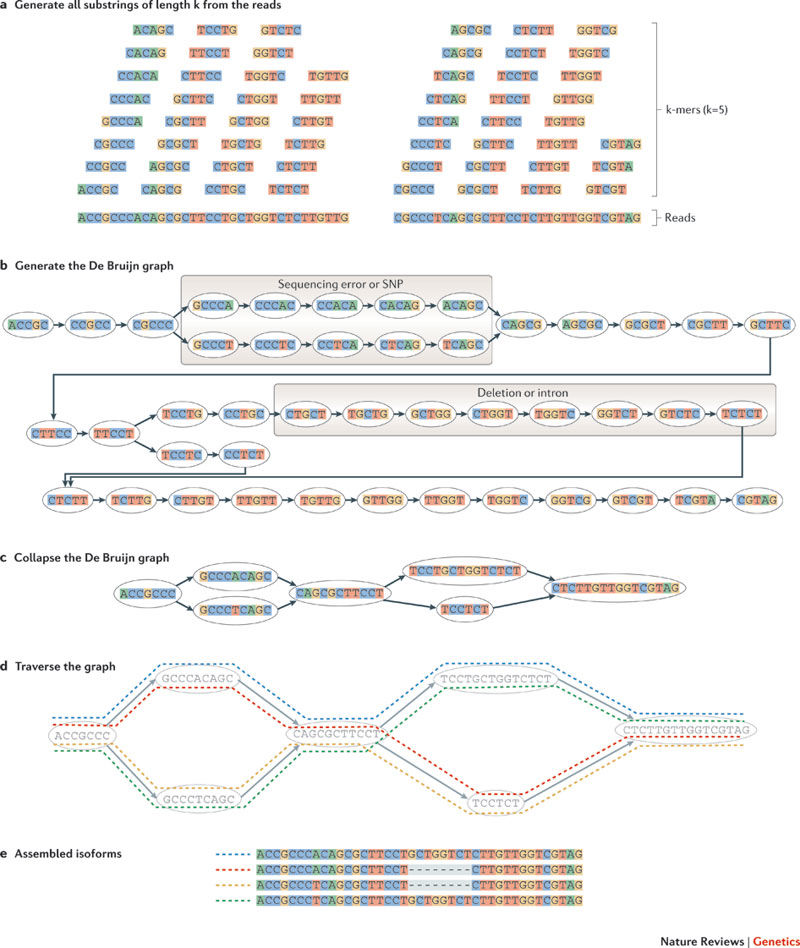
\includegraphics[height=7cm]{Images/denovo.jpg}
\end{column}
\begin{column}{0.48\textwidth}
\begin{itemize}
  \scriptsize
  \item a) all substrings of length k (k-mers) are generated from each read
  \item b) each unique k-mer is used to represent a node in the De Bruijn graph,pairs of nodes are connected if shifting a k-mer by one character creates an exact k???1 overlap between the two k-mers. 
  \item The example (5-mers) illustrates a SNP or sequencing error and an example of an intron or a deletion. 
  \item Single-nucleotide differences cause 'bubbles' of length k in the De Brujin graph, whereas introns or deletions introduce a shorter path in the graph
  \item c,d) chains of adjacent nodes in the graph are collapsed into a single node when the first node has an out degree of one and the second node has an in degree of one
  \item e) the isoforms are then assembled. See more \href{JA Martin, Z Wang, Nature Reviews Genetics, 2011}{http://rdcu.be/zSpz}
\end{itemize}
\end{column}
\end{columns}
\end{center}
\end{frame}

% de-novo: overview: annotations
\subsection{Annotations of transcripts}
\begin{frame}
\begin{displayquote}
\footnotesize
If a reference genome is available, annotation is relatively straightforward:  genomic coordinates from the reference genome are normally associated with various forms of annotation information through databases. A transcriptome assembled de novo, on the other hand, is often annotated from scratch
\end{displayquote}
\begin{block}{NCBI-supported BLAST}
\begin{itemize}
\footnotesize
  \item "match" query sequences to one or more databases of curated, annotated sequences, using an efficient local sequence alignment approach.
  \item it may be adequate to blast against a database of known or predicted transcripts from the reference genome of a closely-related organism
  \item it may be desirable to blast contigs against all nucleotide sequences in an inclusive database
  \item if the annotation emphasis is on protein-coding transcripts, BLASTx, which translates each query sequence (in all six reading frames) to amino acid sequences and uses these to query a protein database, may be an appropriate tool
\end{itemize}
\end{block}
\end{frame}

\section{And what about scRNA-seq?}
\section{Summary}

\section{Exercises}
\subsection{Main exercise}
\begin{frame}
\begin{block}{Main exercise}
\begin{itemize}
\item checking the quality of the raw reads with FastQC
\item mapping the reads to the reference genome using STAR
\item converting between SAM and BAM files format using Samtools
\item assessing the post-alignment reads quality using QualiMap
\item counting reads overlapping with genes regions using featureCounts
\item building statistical model to find DE genes using edgeR called from a prepared R script
\end{itemize}
\end{block}
\end{frame}

% Exercise 2
\subsection{Bonus exercises}
\begin{frame}
\begin{block}{Bonus exercises}
\begin{itemize}
\item functional annotation, putting DE genes in the biological context
\item exon usage, studying the alternative splicing
\item data visualisation and graphics
\item de novo transcriptome assembly
\end{itemize}
\end{block}
\end{frame}
  

\begin{frame}
\begin{center}
\huge
Thank you for attention \newline
\vspace{1cm}
Questions? \newline
\vspace{1cm}
Enjoy the rest of the course
\end{center}

\begin{block}{Read more}
\begin{itemize}
  \item RNA-seqlopedia
  \item RNA-Seq blog
  \item Conesa et al. Genome Biology, 2016, A survey of best practices for RNA-seq data analysis
\end{itemize}
\end{block}
\end{frame}


\end{document}
